\chapter{Machine Learning for HEP}
\label{sec:03_ml}

\section{Introduction}

Machine learning (ML) and deep learning (DL) are revolutionizing data analysis, computing, and even real-time triggers in high-energy physics (HEP).
Significant contributions of this dissertation include ML advancements for Higgs boson searches and beyond and fast detector simulations for the HL-LHC.
In this chapter, to motivate them, we introduce some core concepts of ML, especially as they relate to HEP applications.

% In this chapter, we provide a brief introduction to ML in HEP.
ML refers to a general class of algorithms that ``learn'' from data to solve problems.
This is in contrast to traditional, hand-engineered bespoke algorithms designed by domain experts to address specific tasks.
A relevant example in HEP is selecting a high-purity, in terms of signal versus background, region of data: a traditional approach would be to manually define a set of selections on individual kinematic features based on physical reasoning; for example, when measuring Higgs boson production, we select for events exhibiting resonances around the Higgs mass.

However, as we enter the regime of extremely large quantities of high-dimensional data and measurements of ever more complex processes (such as the \HH searches described in this dissertation), it soon becomes intractable, or at least suboptimal, to manually define selections over the $\mathcal O$(10--100) event features that can help distinguish signal from background.
This is where we turn to ML algorithms, such as boosted decision trees (BDTs)~\cite{hastie2009boosting}, which can automatically compute optimal, non-linear selections in this high-dimensional feature space.

More recently, the advent of artificial neural networks (ANNs) and deep learning (DL), along with increased data availability and computing power, has led to orders of magnitude increases in the dimensionality of data that can be exploited and the complexity and expressivity of the models built.
A relevant example of their significant impact in HEP is in jet identification: jets are extremely high-dimensional objects, composed of hundreds of particles, tracks, and vertices each with several distinguishing features.
Traditionally, this information had to be aggregated into hand-engineered, high-level features, such as the jet mass, number of prongs, and vertex displacements.

DL, on the other hand, allows us to leverage the full set of low particle- and vertex-level features.
This leads to powerful classifiers that significantly outperform traditional methods and improve the sensitivity of our jet-based measurements.
This is exemplified by the new \HVV jet identification algorithm we introduce in Chapter~\ref{sec:05_jet_tagging} and apply to searches for \HH production in Chapter~\ref{sec:05_hh}.
As we argue in Section~\ref{sec:03_genaes}, DL also has the potential to alleviate the computational challenges we foresee in the HL-LHC era, particularly with respect to detector simulations, which are the focus of Part~\ref{part:ml4sim}.

ANNs have proven to be extremely flexible building blocks out of which to construct diverse and sophisticated models for a variety of tasks in HEP, from classification and regression to simulation and anomaly detection, and more.
Indeed, the development of DL algorithms in HEP is a rapidly growing subfield in its own right, and its various applications are visualized as a ``nomological net'' in Figure~\ref{fig:03_ml_nomological_net}; a comprehensive ``living'' review is available in Ref.~\cite{hepmllivingreview}.
As we discuss below, however, with more complex data and models also comes the need for more sophisticated methods to validate, calibrate, and trust them; this is the subject of Chapters~\ref{sec:04_evaluating} and~\ref{sec:05_hww_calibration}, on evaluating generative models and calibrating \HVV jet taggers, respectively.

In this chapter, we first provide a brief introduction to ML and DL, emphasizing key aspects relevant to HEP.
These include the importance of: 1) generalization and calibration of models trained on simulations (Section~\ref{sec:03_ml_calibration}); and 2) the importance of building thoughtful, physics-informed models and representations for our data (Section~\ref{sec:03_ml_physics}).
In the same spirit, we then discuss \textit{equivariant neural networks} in Section~\ref{sec:03_ml_equivariantnns}, which are designed to respect the symmetries of physical data, such as Lorentz transformations in HEP.
Finally, we detail two types of unsupervised learning algorithms, autoencoders and generative models, that are relevant to the work in this dissertation in Section~\ref{sec:03_genaes}.

\begin{figure}[ht!]
    \centering
    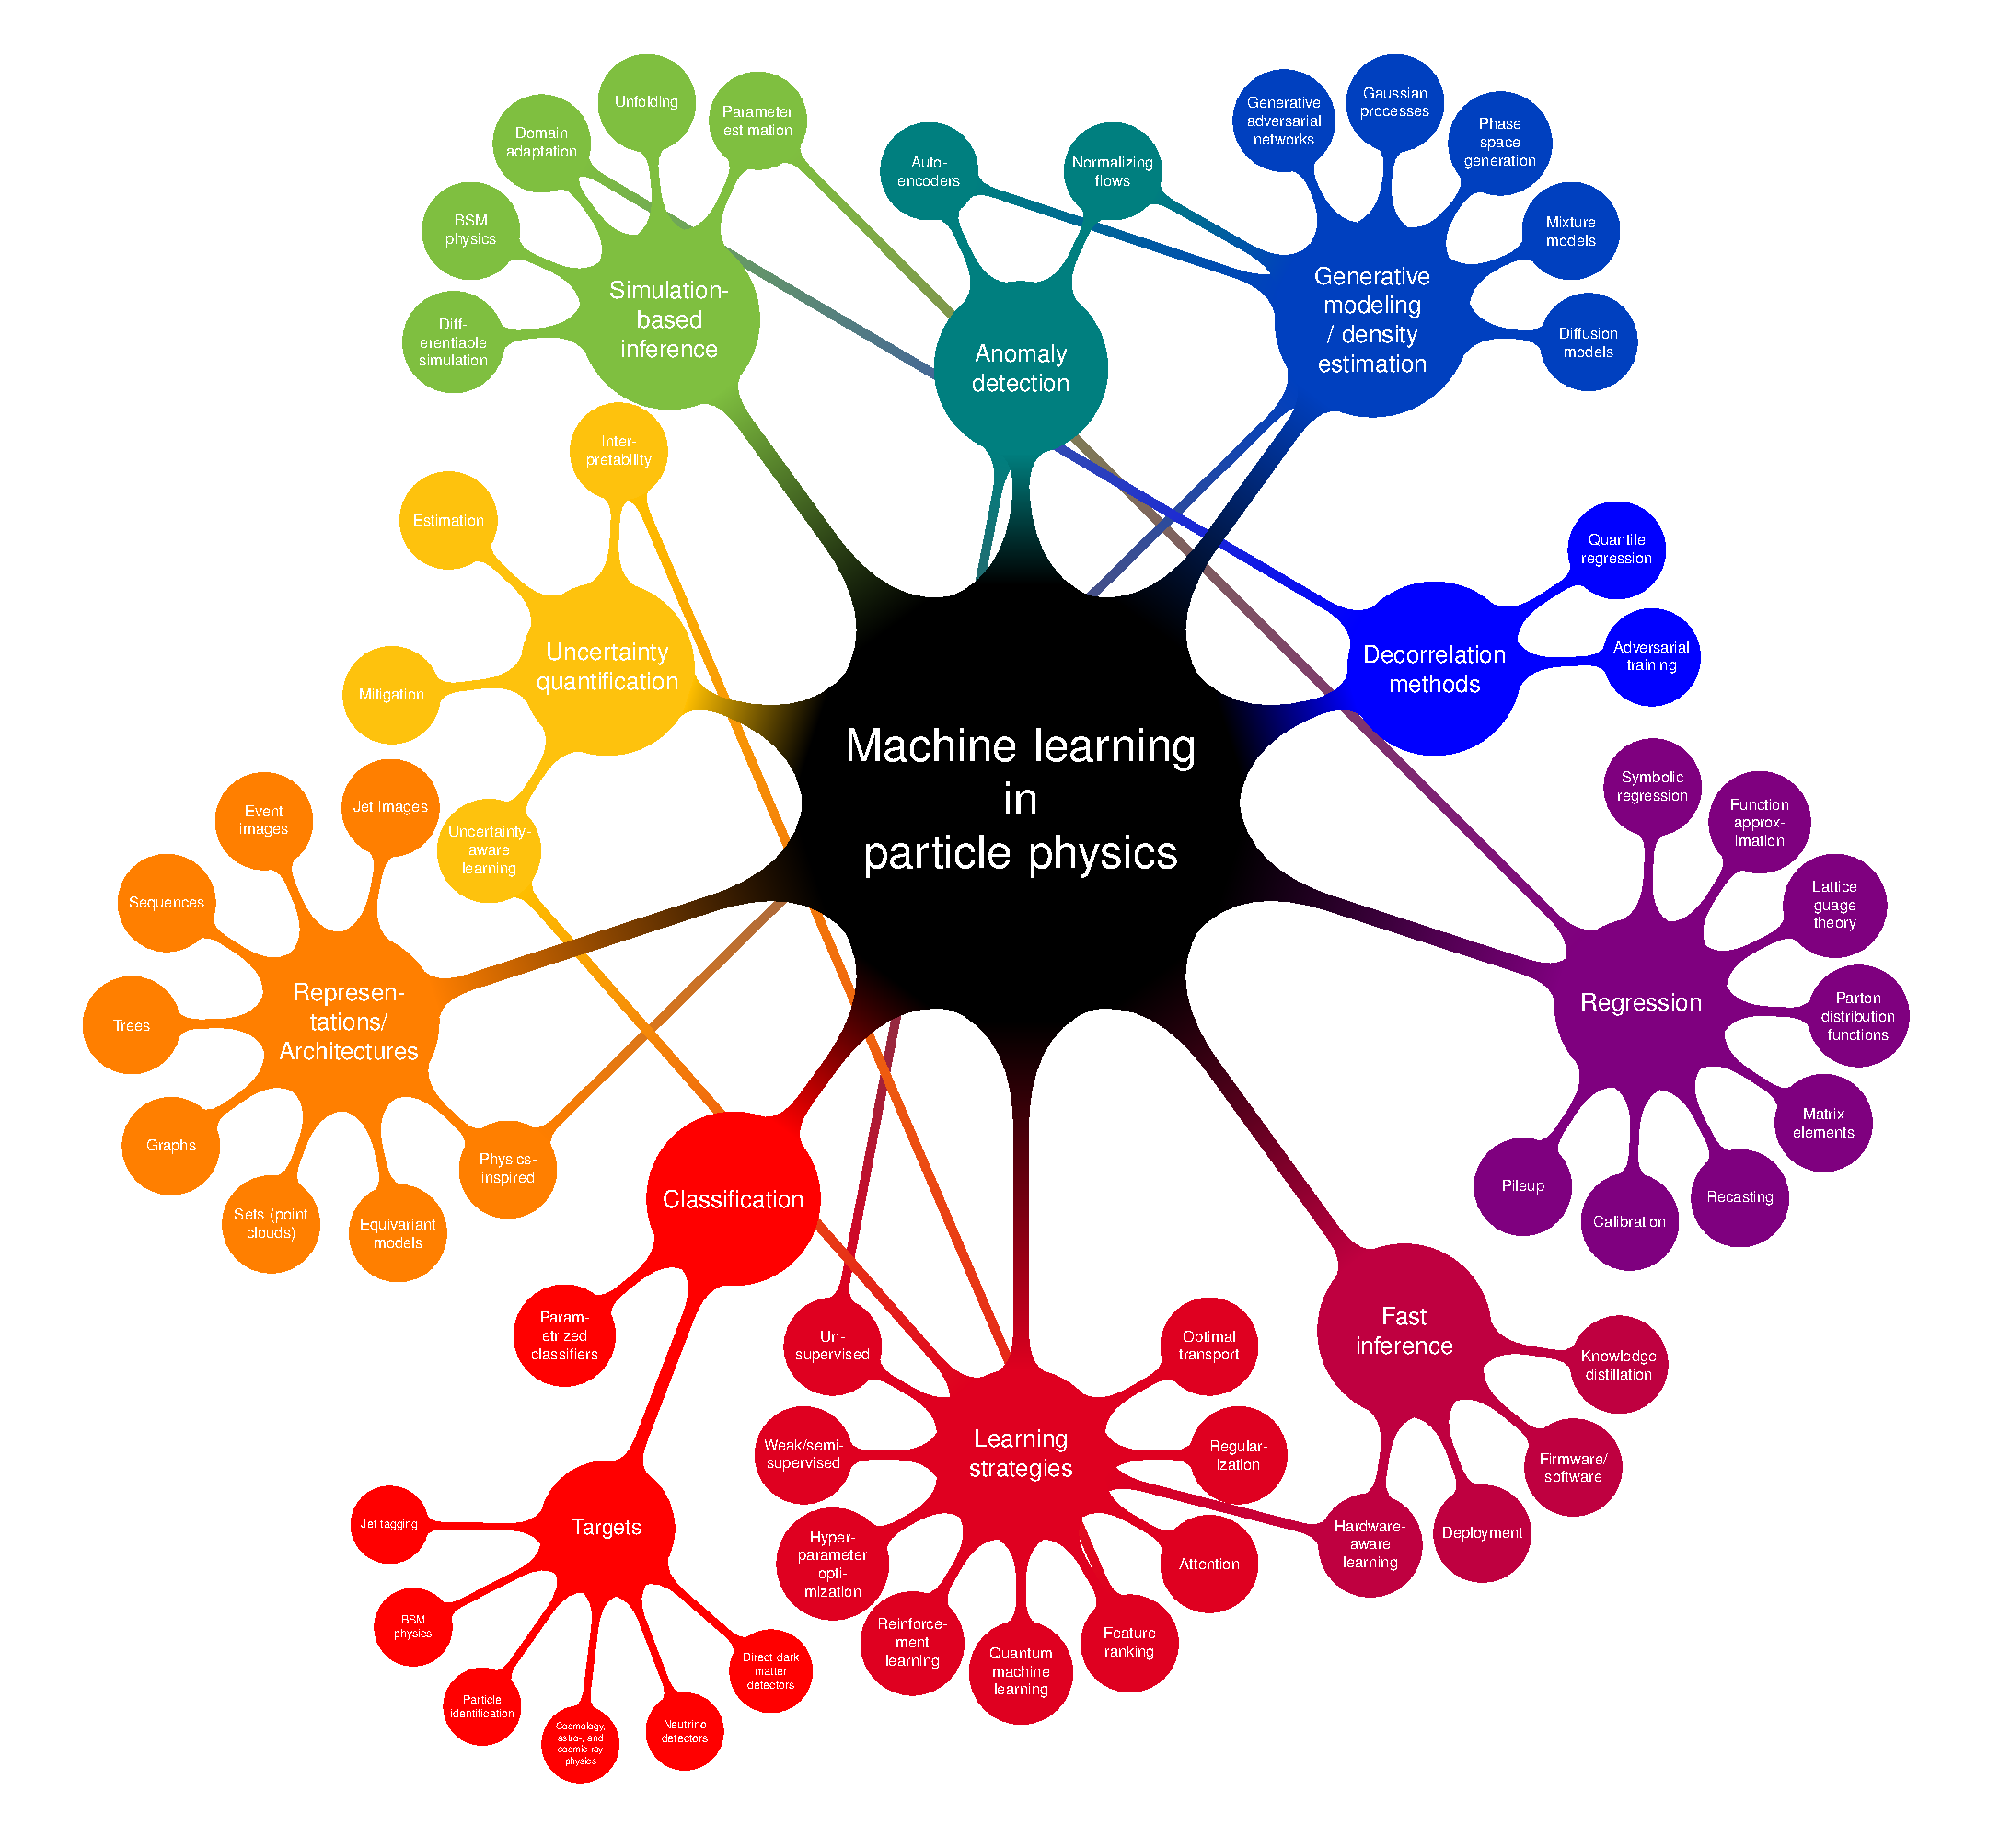
\includegraphics[width=\textwidth]{figures/03-ML/nomological_net}
    \caption{A ``nomological net'' of ML applications in HEP, reproduced from Ref.~\cite{lincoln2024instrumentation}.}
    \label{fig:03_ml_nomological_net}
\end{figure}

\subsection{Basics of ML}
\label{sec:03_ml_basics}

\subsubsection{Supervised and unsupervised learning}

ML algorithms can be broadly categorized as \textit{supervised} and \textit{unsupervised} learning.
The former involves learning a mapping between some input data ${\cvec{x}}$ and a specific output $\cvec{y}$; for example, classifying jets as originating from a Higgs boson or QCD background.
Other examples include regression tasks where the target output is a continuous variable, such as predicting the mass of a jet or the energy of a particle.
Algorithms used for supervised learning include support vector machines (SVMs)~\cite{cortes1995support}, (boosted) decision trees (BDTs)~\cite{breiman1984classification, hastie2009boosting}, and neural networks.
Such algorithms necessitate a \textit{labeled} training dataset of input-output pairs $(\cvec{x}_i, \cvec{y}_i)$.

Tasks for which we do not have straightforward labeled data are considered unsupervised learning problems, in which the model must learn the properties and structure of the data $\cvec{x}$ without explicit target outputs.
Examples include clustering algorithms, which aim to group similar data points together, and generative and anomaly detection models, both of which aim to learn the underlying distribution of the data in some manner for the purposes of generating new data or identifying outliers, respectively.
The latter two will be discussed in more detail in Section~\ref{sec:03_genaes}.

Note that these two categories are not mutually exclusive but rather two ends of a spectrum, with the middle ground including paradigms such as weakly-supervised~\cite{chapelle2006semisupervised} and self-supervised learning~\cite{balestriero2023cookbookselfsupervisedlearning}.

\subsubsection{Linear models}

Perhaps the simplest example of an ML task is linear regression, which entails fitting a linear model:
\begin{equation}
    \label{eq:03_ml_linear}
    f(x|w) = \cvec{w} \cdot \cvec{x}
\end{equation}
to a set of data points $(\cvec{x}_i, y_i)$, where $\cvec{w}$ are the model \textit{weights} which need to be learned.
%  and are the parameters ``learned'' during the training.
To do so, we define a \textit{loss function} $L$ that quantifies the difference between the model's prediction and our desired output, such as the mean squared error:
\begin{equation}
    \label{eq:03_ml_mse}
    L = \frac{1}{N} \sum_{i=1}^N (f(x_i|w) - y_i)^2.
\end{equation}
The learning objective of our model is hence to minimize $L$ with respect to the weights $\cvec{w}$.

For linear regression, the minimum can in fact be found analytically to be:
\begin{equation}
    \label{eq:03_ml_linear_soln}
    \cvec{w} = (\cvec{X}^T \cvec{X})^{-1} \cvec{X}^T \cvec{y},
\end{equation}
where $\cvec{X}$ is the matrix of input data and $\cvec{y}$ the vector of target outputs.
However, for more complex models (or even in linear regression when the matrix inversion is too expensive), numerical optimization techniques are required.
The most common is \textit{gradient descent}.

\subsubsection{Gradient descent}

Gradient descent is an optimization algorithm that iteratively adjusts the weights of a model in the direction of steepest descent, i.e., the gradient:
\begin{equation}
    \label{eq:03_ml_grad_desc}
    \cvec{w}_{t+1} = \cvec{w}_t - \eta \nabla_w L,
\end{equation}
where $\cvec{w}_t$ are the weights at iteration $t$, and $\eta$ is the step size or \textit{learning rate} (LR).
This process is visualized for two learnable parameters in Figure~\ref{fig:03_ml_gradientdescent}.

\begin{figure}[ht]
    \centering
    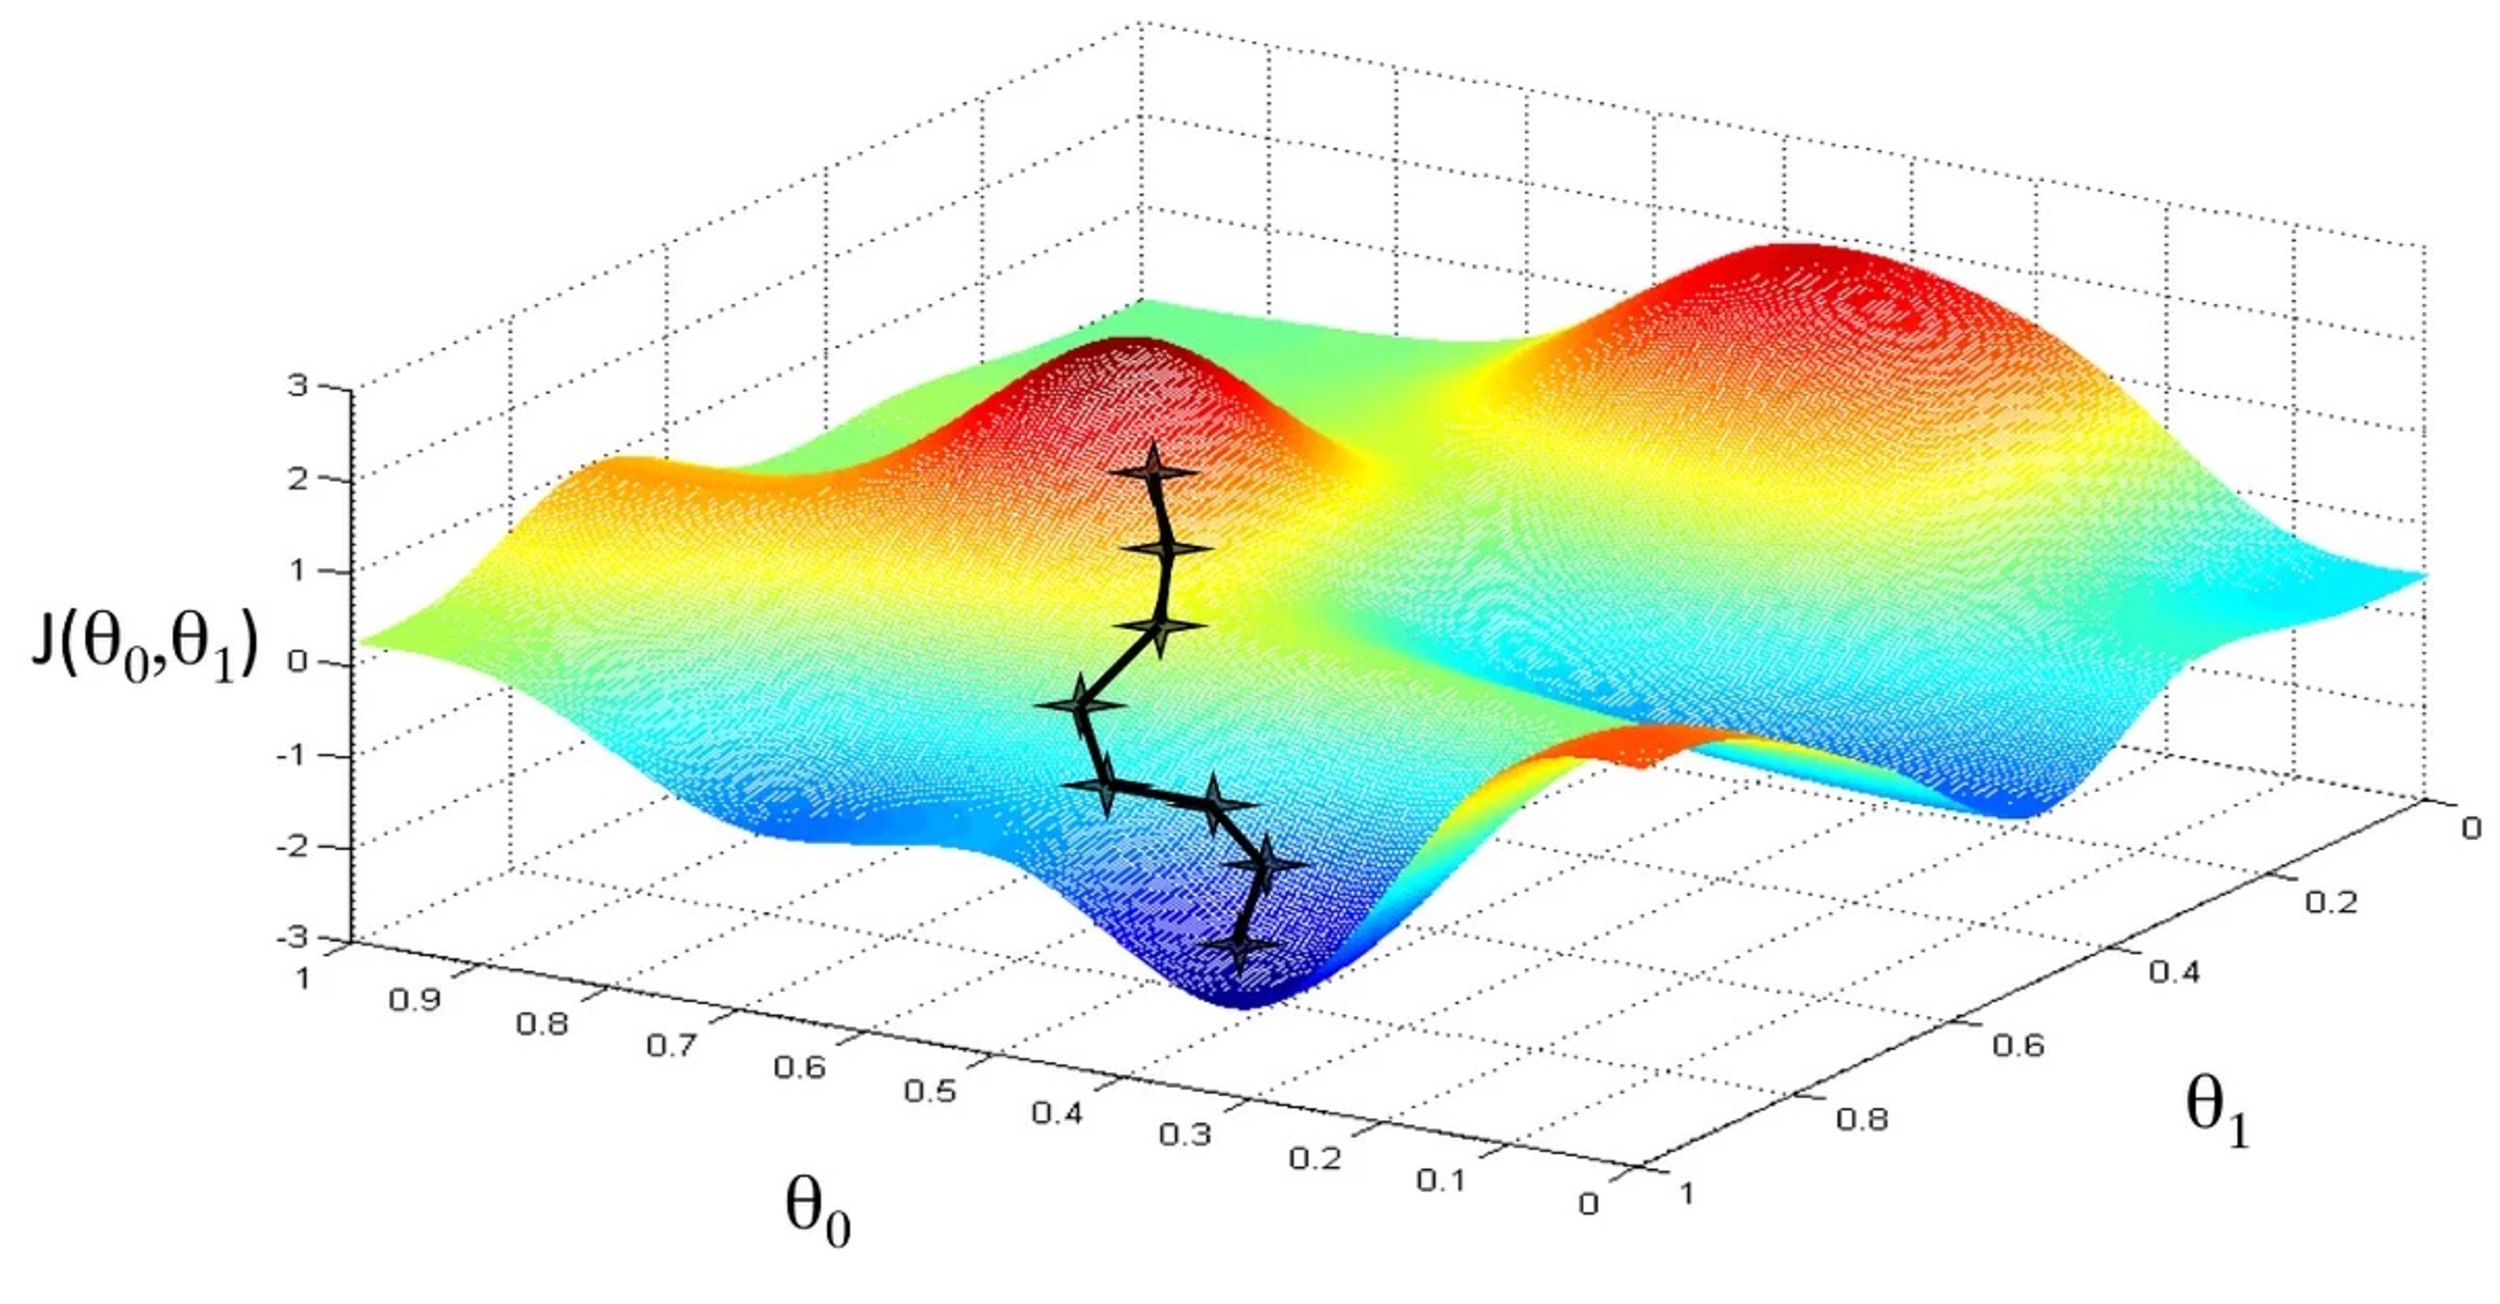
\includegraphics[width=0.6\textwidth]{figures/03-ML/gradientdescent}
    \caption{Illustration of gradient descent in a 2D parameter space of $(\theta_0, \theta_1)$.}
    \label{fig:03_ml_gradientdescent}
\end{figure}

Gradient descent is the backbone of all deep learning optimization algorithms; though this basic idea is typically modified to improve convergence and efficiency.
The most common variants are \textit{stochastic} and \textit{mini-batch} gradient descent, which compute the gradient on a subset of the data at each iteration.
This has the dual benefit of computational efficiency and the introduction of stochasticity into the optimization process, which can help the model escape local minima of the loss function.

Other powerful ideas include \textit{adaptive learning rates}, which adjust the LR during training based on the history of the gradients and/or number of iterations; and \textit{momentum}, which retains some fraction of the previous gradients to smooth out oscillations in the optimization process.
Popular optimizers which incorporate these techniques include RMSprop~\cite{hinton2012rmsprop} and Adam~\cite{kingma2015adam}, both of which are prominently used for the work in this dissertation.

\subsection{The importance of generalization and calibration}
\label{sec:03_ml_calibration}

It is crucial in ML that the model not only learns the training data but can also \textit{generalize} to new, unseen data.
This is what signifies that the model has effectively learned the underlying patterns and relationships, rather than merely memorizing, or \textit{overfitting} to, the training samples.

A standard procedure to evaluate generalization is to split the available dataset into three subsets: training, validation, and testing.
The former is the only dataset used to update the learnable parameters of the model themselves, and is typically the largest subset.
The validation set is used to tune \textit{hyperparameters} of the model --- those parameters such as model size and learning rates that cannot be ``learned'' through gradient descent --- as well as assess the model's performance on unseen data during training: if the performance on the validation set is significantly worse than on the training set, the model is likely overfitting.
Finally, in case a bias is introduced by tuning the hyperparameters on the validation set, it is good practice to evaluate the model on the testing set at the end, which is never used to make decisions on the model.

\subsubsection{The bias-variance tradeoff}

Selecting the right model and hyperparameters involves making a \textit{bias-variance tradeoff}.
This is a fundamental concept in ML that describes the balance between two sources of error in a predictive model.
\textit{Bias} is the error due to overly simplistic assumptions in the learning algorithm --- for example, using a linear model to capture non-linear relationships; while \textit{variance} is the error due to a model which is too complex capturing noise in the training data.

A model with high bias may have systematic inaccuracies, or \textit{underfit} the data, while a model with high variance may overfit and fail to generalize.
Model selection involves using the performances on the training and validation datasets to find an optimal balance between these two errors.
Common techniques to improve bias include improving the model design and increasing its complexity, while to address variance, there are several established \textit{regularization} methods to reduce overfitting, such as early stopping~\cite{prechelt2012early}, dropout~\cite{srivastava2014dropout}, and batch normalization~\cite{ioffe2015batch}.


\subsubsection{Model calibration}

A related and unique aspect of ML in HEP is the reliance on theory and detector simulations to generate large quantities of labeled data for model training.
The aim though, of course, is to deploy on and model correctly the real data collected by the experiments.
It is hence crucial to verify how well the models generalize accurately to the latter, rather than overfitting to mismodeling in the former.

This process is sometimes referred to as \textit{calibration}, where the performance of the ML model is compared between simulation and data to derive possible corrections to the model's predictions and quantify the systematic uncertainties associated with them.
As models become more complex and high-dimensional, calibration becomes increasingly challenging (and often overlooked)!
To this end, significant contributions of this dissertation are the development of novel methods to efficiently and sensitively validate the performance of ML-based simulations (Chapter~\ref{sec:04_evaluating}), and improving the calibration of \HVV jet identification algorithms (Chapter~\ref{sec:05_jet_tagging}).


\subsection{Artificial neural networks and deep learning}

ANNs are ML models loosely inspired by the structure of the human brain.
They were originally proposed in the 1940s, and improved over the 20th century through the perceptron~\cite{rosenblatt1958perceptron} and backpropagation~\cite{rumelhart1986learning} algorithms, but had limited success in practical applications compared to algorithms like SVMs and decision trees.

Only in the 2010s was it recognized that their flexibility in both architecture and training makes them ideal for exploiting the recent exponential increase in data and computing power, propelling ANNs to the forefront of ML and sparking the so-called DL revolution.
% Only during the last decade have they been propelled to the forefront of ML, as their flexibility in both architecture and training turned out to make them ideal for exploiting the recent exponential increase in data and computing power.
Through the development of large and innovative, so-called \textit{deep} neural networks (DNNs), they have led to significant breakthroughs in the fields of computer vision, natural language processing, and indeed HEP.
% A big advantage of NNs is that they are flexible structures that can be used to build a diverse range of deep learning (DL) models for different tasks and data types.
Specific types of models, or ``architectures'', include convolutional neural networks (CNNs) for image data, graph neural networks (GNNs) for graph data, and transformers for sets and sequences, all of which we discuss below.

\subsubsection{Artificial neurons and multilayer perceptrons}

The building blocks of ANNs are single ``artificial neurons'', or \textit{perceptrons}~\cite{rosenblatt1958perceptron}.
They are similar to the linear models discussed above, but with an additional non-linear function $\sigma$ --- known as the \textit{activation function}, applied to the output (Figure~\ref{fig:03_ml_perceptron}, left):
\begin{equation}
    \label{eq:03_ml_perceptron}
    f(x|w, b) = \sigma(\cvec{w} \cdot \cvec{x} + b),
\end{equation}
where $b$ is a constant, learned \textit{bias} term.
Common choices for the activation include the sigmoid, hyperbolic tangent, and piecewise linear functions.

By combining multiple perceptrons in a \textit{multilayer perceptron} (MLP) architecture, i.e., an ANN, we can build a powerful and flexible model capable of learning complex, non-linear relationships in the data (Figure~\ref{fig:03_ml_perceptron}, right).
In fact, the famous \textit{universal approximation theorem}~\cite{hornik1989multilayer} states that, in theory, neural networks can approximate any continuous function to arbitrary accuracy given a sufficiently large number of neurons and layers (although in practice it is not so straightforward).

\begin{figure}[ht]
    \centering
    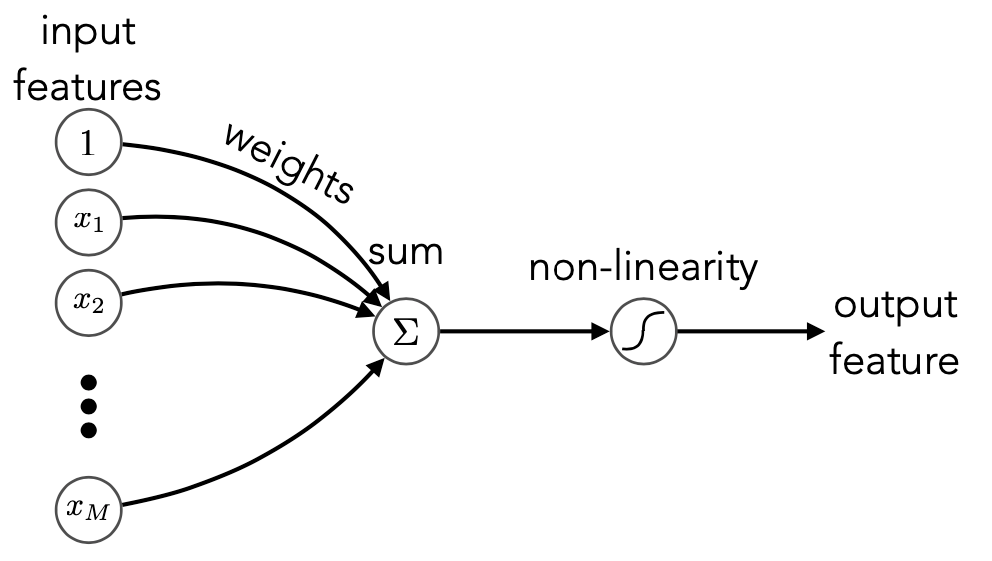
\includegraphics[width=0.49\textwidth]{figures/03-ML/perceptron}
    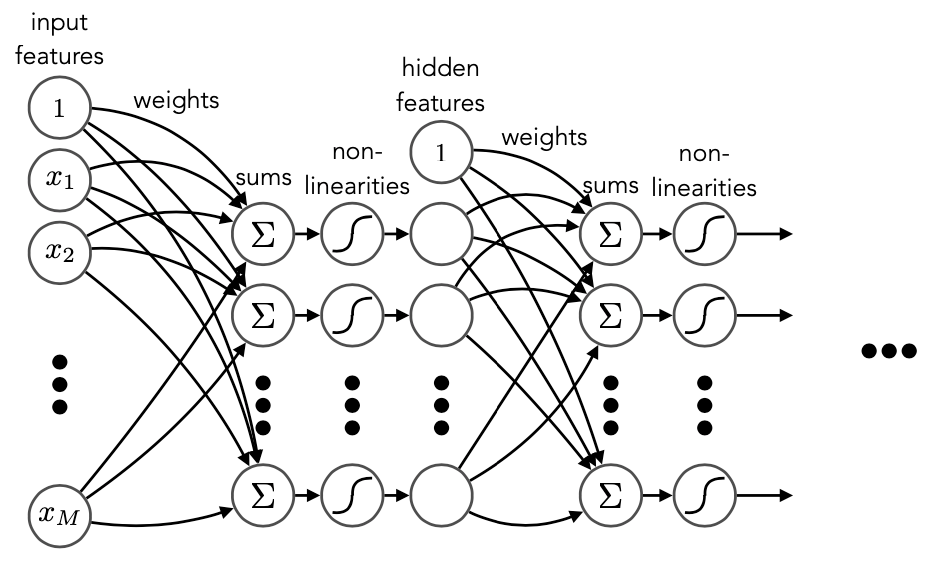
\includegraphics[width=0.49\textwidth]{figures/03-ML/nn}
    \caption{(Left) a single perceptron and (right) a neural network built using multiple layers of perceptrons (MLPs).}
    \label{fig:03_ml_perceptron}
\end{figure}

Another key characteristic of ANNs is their ability to learn hierarchical representations of the data, with each layer, in principle, learning progressively more abstract features from the previous layer's output.
Intelligently designed ``deep'' networks with many layers can hence learn powerful, nonlinear, high-level representations of the high-dimensional input data, which can then be used to perform the desired task (assuming enough data and computing power to train them effectively).
This is why this subfield of ML is also sometimes referred to as \textit{representation learning}.
As we discuss in Section~\ref{sec:03_ml_physics}, it is thus crucial to use representations and design architectures well-suited to the data and task at hand; naively adopting a specific architecture or input representation from another domain may not lead to the most optimal feature learning.


\subsubsection{Backpropagation}

Part of the effectiveness and popularity of DNNs is due to the backpropagation algorithm~\cite{rumelhart1986learning}, which allows for efficient training of arbitrarily deep networks.
Backpropagation is, essentially, the repeated application of the chain rule of calculus to iteratively propagate gradients of the loss function backwards through the network.
For a simple two-layer network, for example:
\begin{equation}
    \label{eq:03_ml_backprop_nn}
    f(x|w, b) = \sigma^{(2)}(\cvec{w}^{(2)} \cdot (\sigma^{(1)}(\cvec{w}^{(1)} \cdot \cvec{x} + \cvec{b}^{(1)}) + \cvec{b}^{(2)}),
\end{equation}
where the superscript denotes the layer of the network, the gradient of the loss function $L$ with respect to $\cvec{w}^{(1)}$ is:
\begin{equation}
    \label{eq:03_ml_backprop}
    \frac{\partial L}{\partial w^{(1)}} = \underbrace{\frac{\partial L}{\partial f} \frac{\partial f}{\partial \sigma^{(2)}} \frac{\partial \sigma^{(2)}}{\partial \cvec{w}^{(2)}}}_{\cnicefrac{\partial L}{\partial w^{(2)}}}
    \underbrace{\frac{\partial \cvec{w}^{(2)}}{\partial \sigma^{(1)}} \frac{\partial \sigma^{(1)}}{\partial \cvec{w}^{(1)}}}_{\cnicefrac{\partial w^{(1)}}{\partial w^{(2)}}}.
\end{equation}
This tells us that $\cnicefrac{\partial L}{\partial w^{(1)}}$ can be computed using the gradient with respect to $w^{(2)}$ --- which needs to be calculated anyway --- and, more generally, by walking backwards through the network operations and taking the product of the derivatives at each step.
This simple but powerful idea scales well to large and diverse network architectures, and is why huge DNNs can be trained effectively with relative ease.

\subsubsection{Convolutional neural networks}

We now walk through some popular ANN architectures, starting with CNNs.
CNNs are a type of NN designed to process grid-like data and, particularly, images.
They contributed the first major breakthrough in DL by achieving impressive performances in computer vision tasks, with models such as AlexNet~\cite{krizhevsky2012imagenet} in 2012 and ResNet~\cite{he2016deep} in 2016.

A single CNN convolutional layer convolves a set of discrete ``kernels'' (essentially, learnable matrices) through the input image or data (Figure~\ref{fig:03_ml_cnn}), each of which detect useful features such as edges or textures.
A CNN comprises multiple convolutional layers, interspersed with operations such as pooling or compression to reduce the spatial dimensions of the data, and then typically MLPs at the end as in Figure~\ref{fig:03_ml_cnn} to produce the final output.

\begin{figure}[ht]
    \centering
    % \captionsetup{justification=centering}
    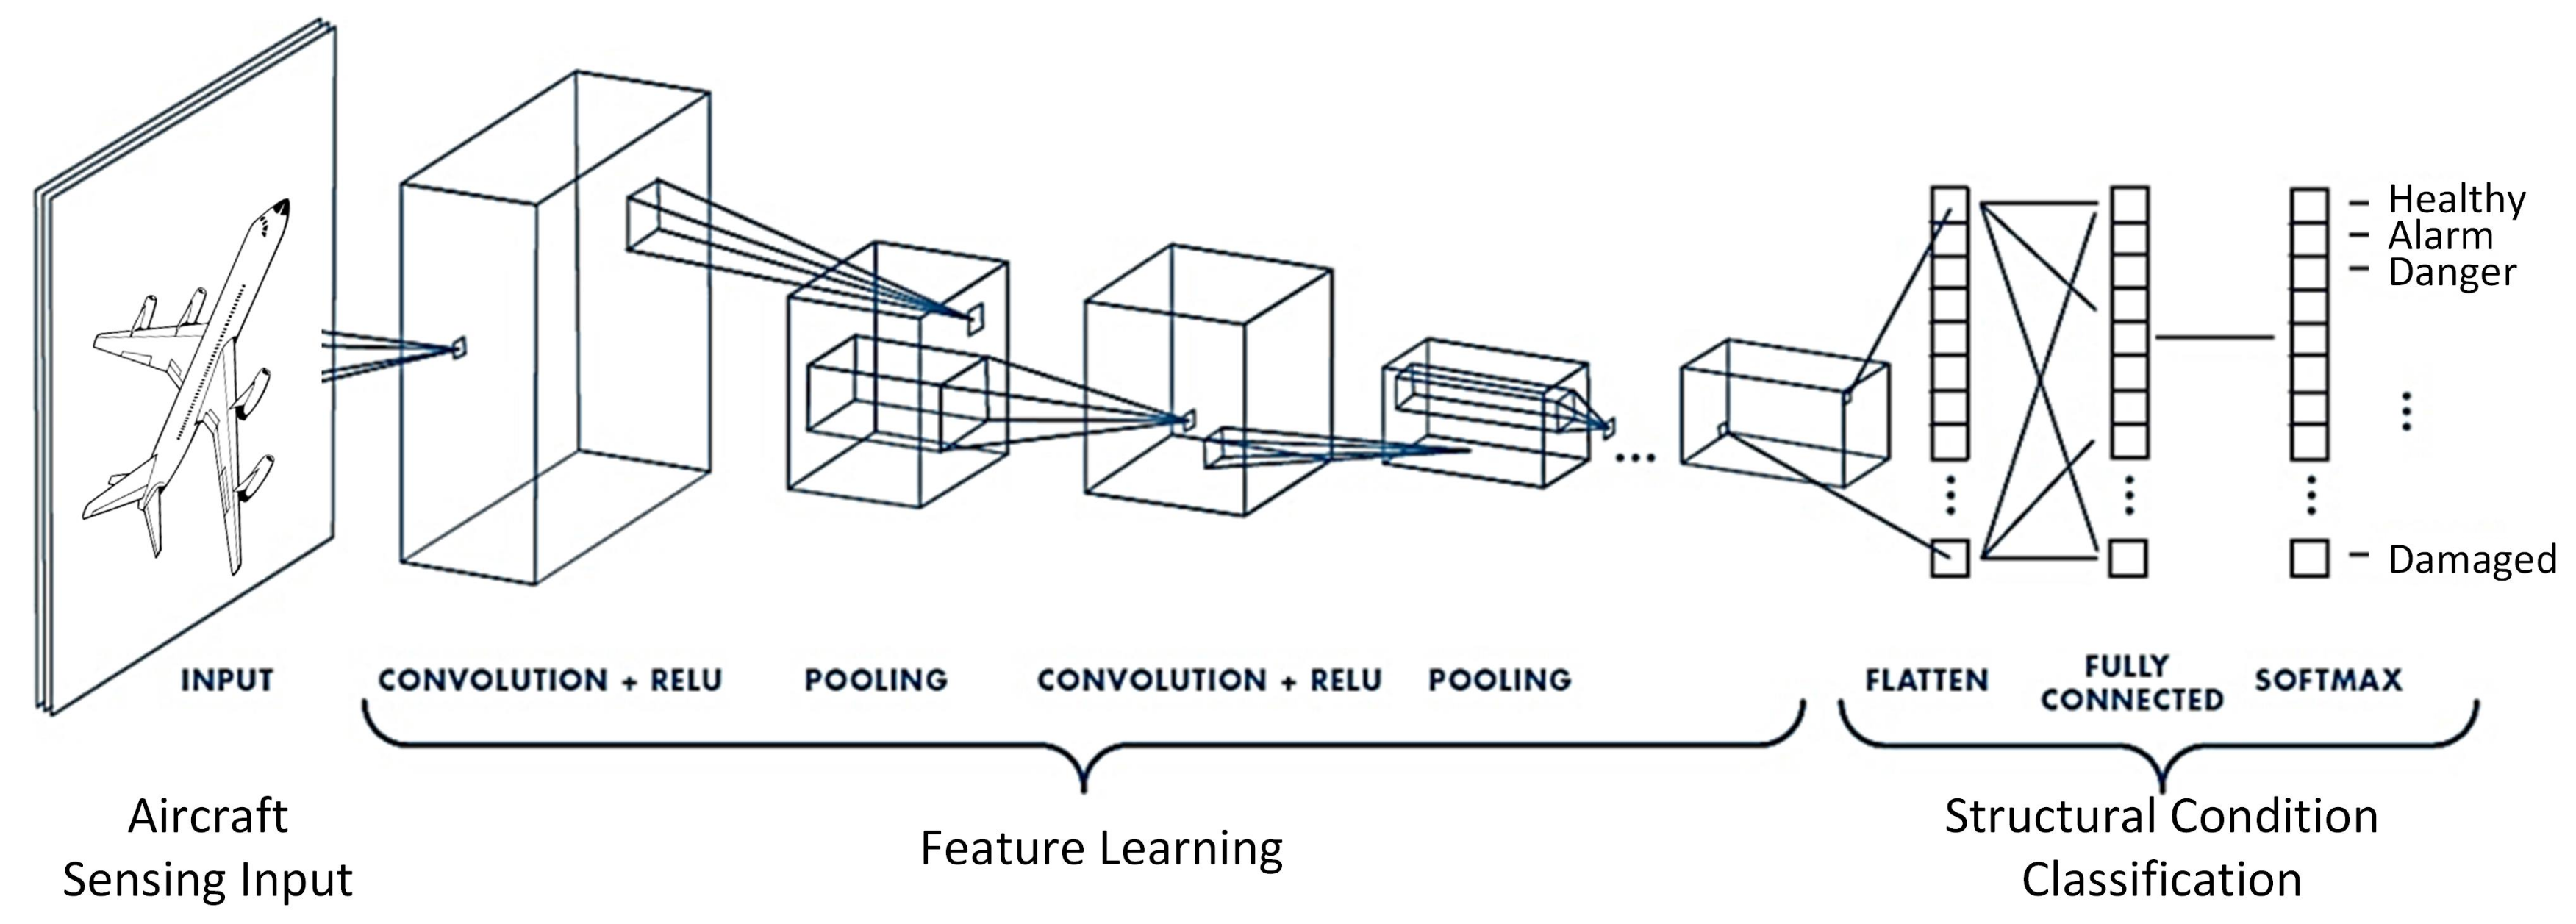
\includegraphics[width=\textwidth]{figures/06-ML4Jets/equivariantnns/sensors-19-04933-g001.png}
    \caption{Schematic of a convolutional neural network, reproduced from Ref.~\cite{iuliana2019convolutional}.}
    \label{fig:03_ml_cnn}
\end{figure}


\subsubsection{Graph neural networks}

GNNs are designed for graph-structured data, such as social networks or molecular structures.
They are also useful for operating on \textit{point clouds}: sets of unordered data points in some space, which we argue in Section~\ref{sec:03_ml_physics} are the perfect data structures for representing particles in an event or hits in a detector.
This is why GNNs have been extremely successful in HEP, generally outperforming standard MLP or CNN approaches.

The idea behind GNNs is to learn representations per-node or per-edge, based on information aggregated from their neighbors.
Some generic methods to do so include local graph convolutions --- similar to CNNs, but with graph-based kernels; and message-passing neural networks (MPNNs), which deliver and aggregate learned messages between nodes.
An example of an MPNN is shown in Figure~\ref{fig:03_ml_gnn}, and is the basis for a novel GNN generative model introduced in Chapter~\ref{sec:04_models}.

\begin{figure}[ht]
    \centering
    \captionsetup{justification=centering}
    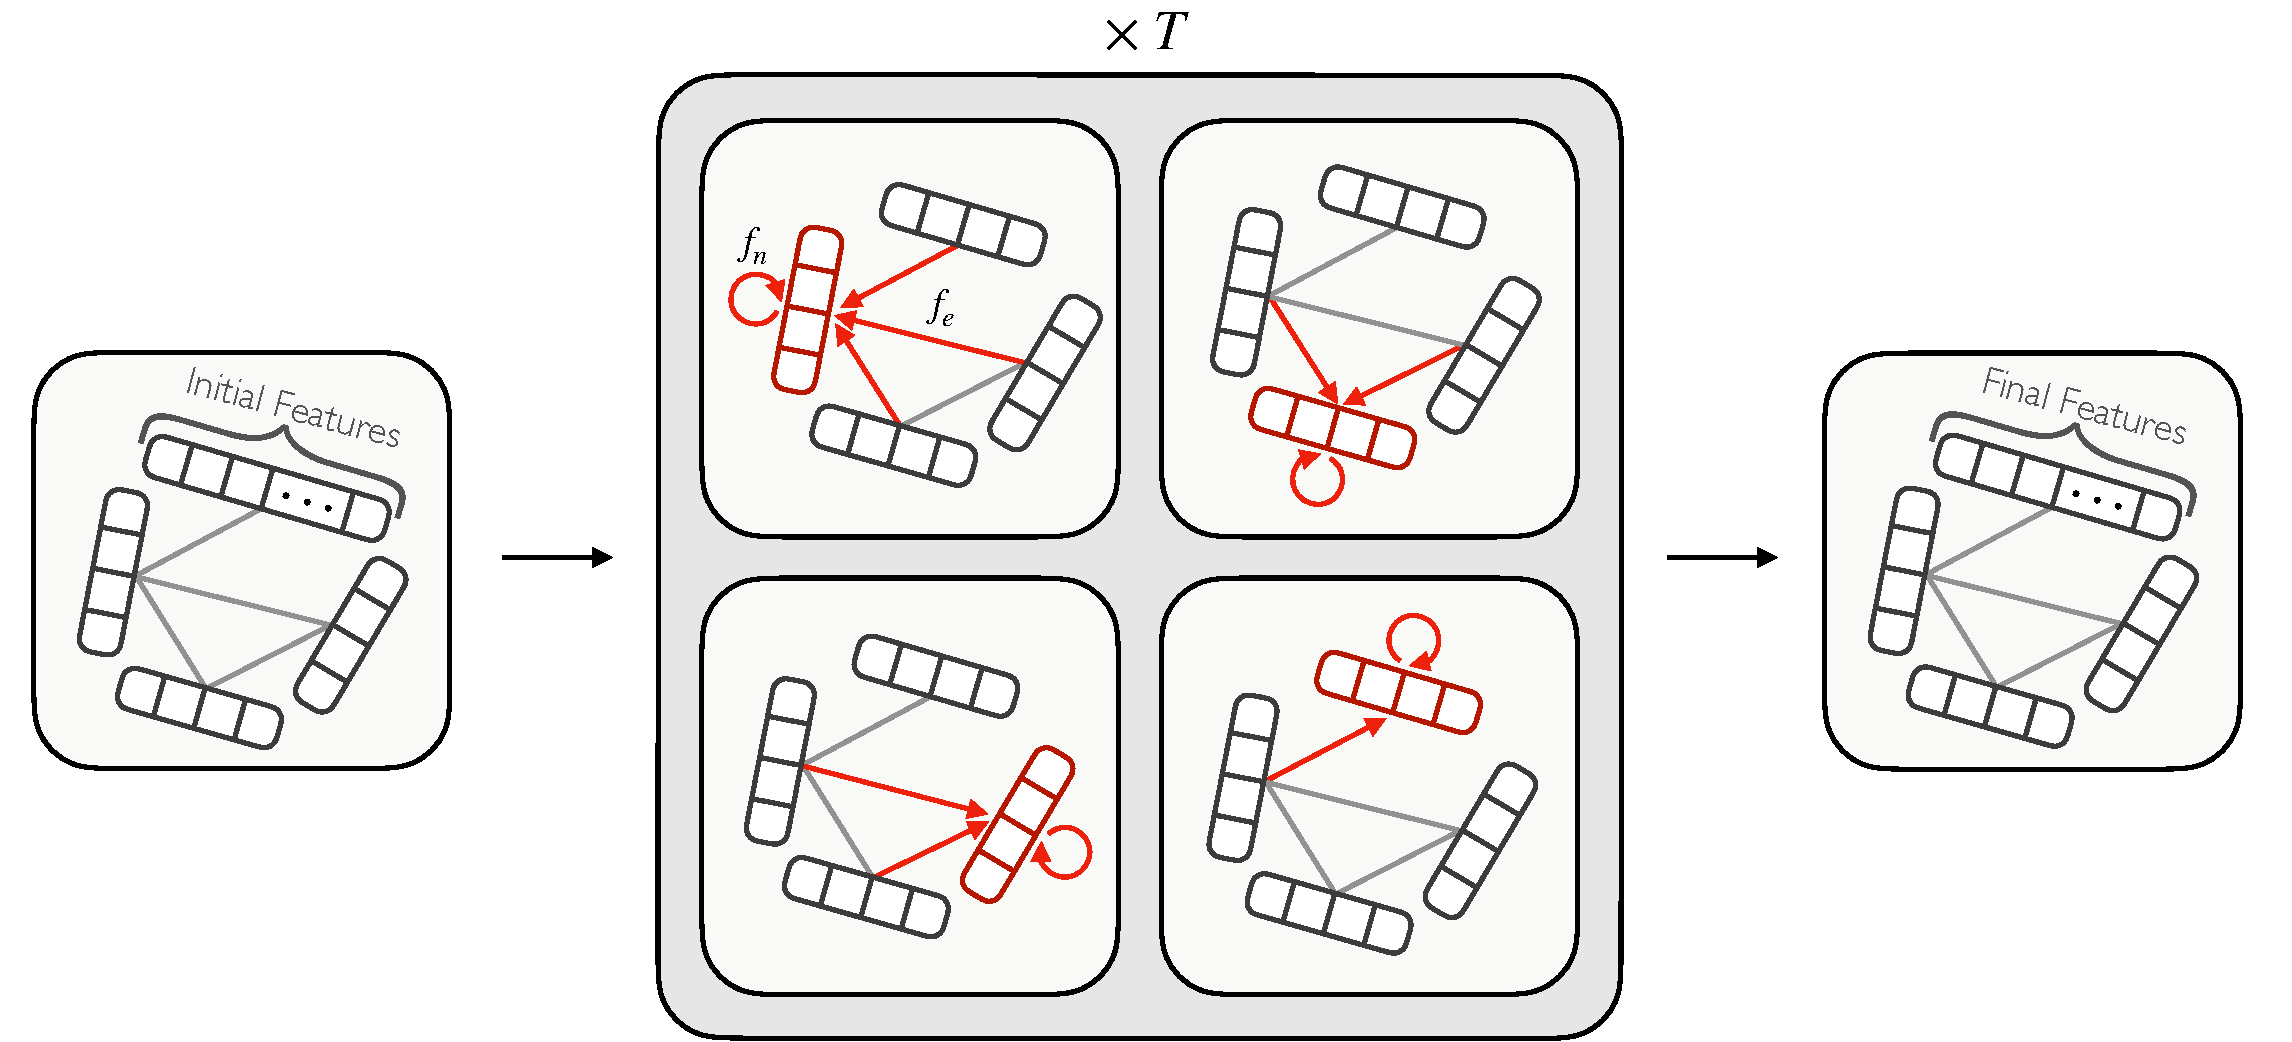
\includegraphics[width=0.7\textwidth]{figures/06-ML4Jets/equivariantnns/mpnn_box_line.pdf}
    \caption{Schematic of a message passing graph neural network.}
    \label{fig:03_ml_gnn}
\end{figure}


\subsubsection{Attention and transformers}

The final architecture we discuss is the transformer, introduced in 2017~\cite{vaswani2017attention}, which is the powerhouse behind the recent revolution in natural language processing (NLP) and AI chatbots such as GPT-3~\cite{brown2020language} and its successors.
Transformers are built around the idea of \textit{attention}, which encourages the model to learn to attend to different parts of an input set or sequence in each layer.

Explicitly, each element, or node's, features in the input set are first embedded via MLPs into \textit{key} ($K$) and \textit{value} ($V$) pairs, while each node in the output set is embedded into a \textit{query} ($Q$).
The attention mechanism is then defined as:
\begin{equation}
    \label{eq:03_ml_attention}
    A(Q, K, V) = \mathrm{softmax}\left(\frac{QK^T}{\sqrt{d_k}}\right)V,
\end{equation}
where $d_k$ is the dimension of the keys and queries, and $\mathrm{softmax}\left(\cnicefrac{QK^T}{\sqrt{d_k}}\right)$ are the ``attention scores'' between each pair of input and output nodes.
This output $A$ is finally used to update the features of the output nodes.
Figure~\ref{fig:04_gapt_attention} shows a schematic of the special case of \textit{self-attention}, in which the input set is also the output set; i.e., each node's features are updated based on the features of all other nodes.

Transformers can be thought of as a type of fully-connected GNN, with attention a (particularly efficient) form of message-passing.
They have proven extremely successful and durable in NLP and other sequence-based tasks, and are also gaining prominence in computer vision and HEP.
We introduce two novel transformer-based models for jet simulations and tagging in Chapters~\ref{sec:04_models} and~\ref{sec:05_jet_tagging}, respectively.

\begin{figure}[ht]
    \centering
    \captionsetup{justification=centering}
    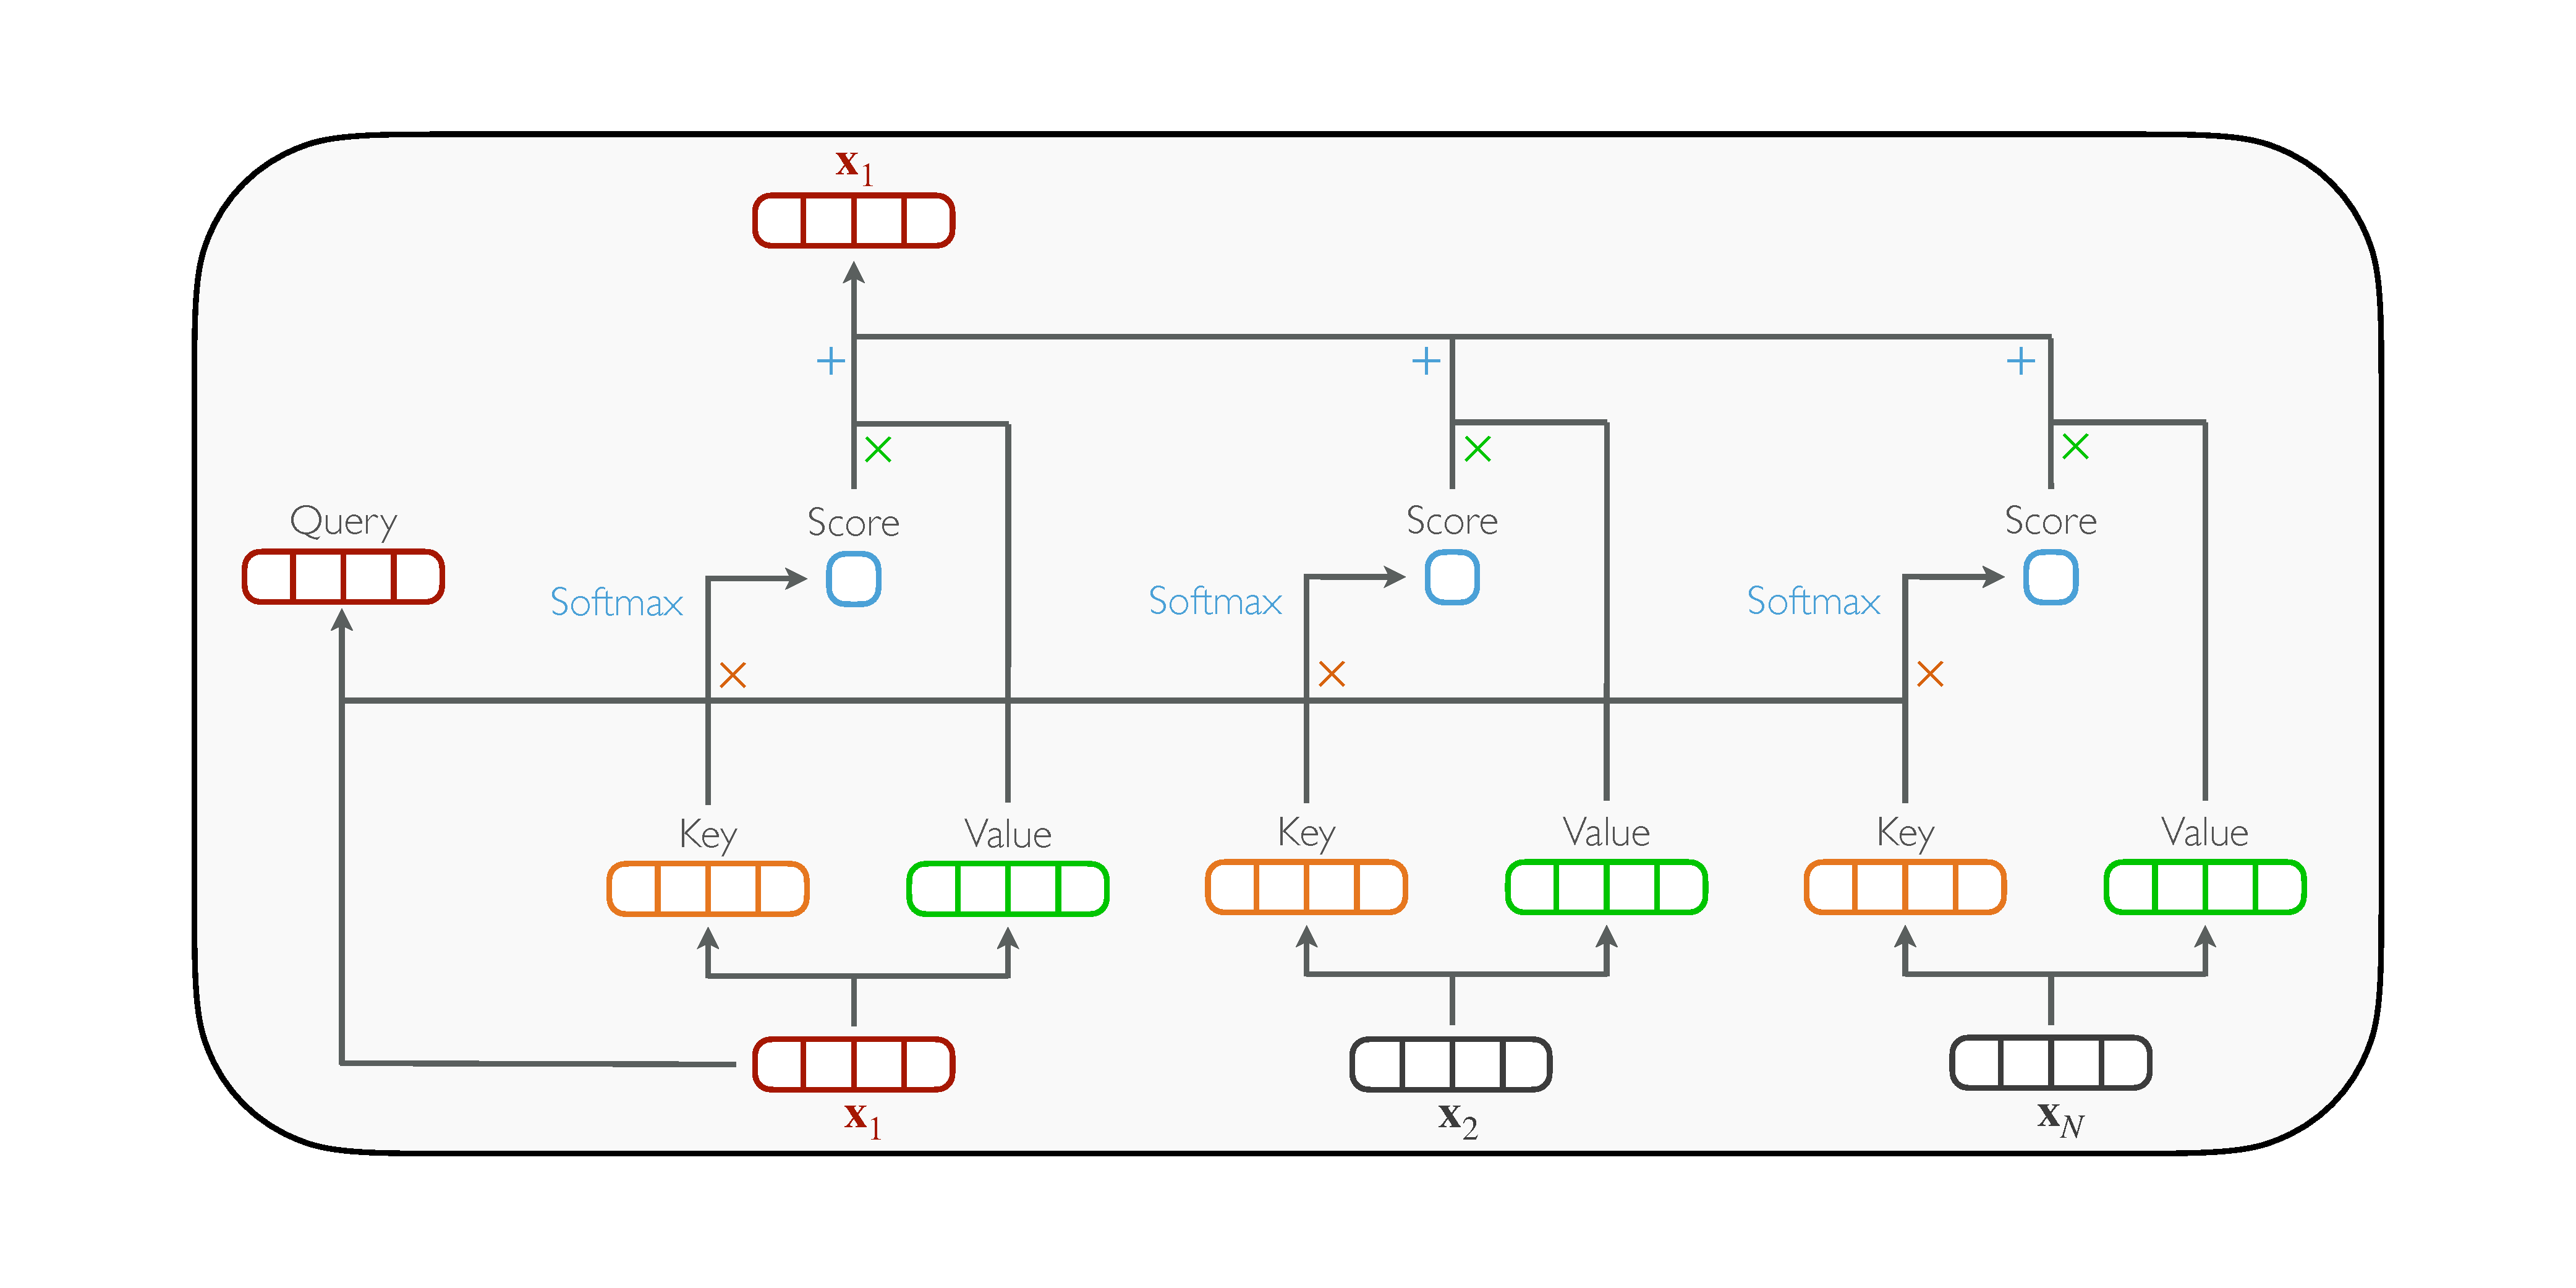
\includegraphics[width=\textwidth]{figures/04-ML4Sim/igapt/attention.pdf}
    \caption{Schematic of set self-attention.}
    \label{fig:04_gapt_attention}
\end{figure}


\subsection{The importance of being physics-informed}
\label{sec:03_ml_physics}

% As highlighted, DNNs have proven extremely powerful in a wide range of tasks.
The success of specific DNN models largely depends on the in-built \textit{inductive biases} --- assumptions or design choices --- towards certain types of data.
This is why it is important in HEP to build physics-informed models and representations that respect the symmetries and biases of our data.
In this section, we outline the relevant properties of HEP data, such as jets and calorimeter showers, and the inductive biases of CNNs, GNNs, and transformers, arguing that the latter two are stronger fits.

The power of CNNs, in addition to their ease of computation, comes from their biases towards natural images, namely: \textit{translation invariance} --- the same features are learned regardless of input translations --- and \textit{locality} --- the convolution operation is inherently local in space, suited to the structure of natural images.
This led to CNNs leading the DL revolution in the 2010s and achieving results on par with or surpassing human performance in computer vision.

Consequently, this also led to early work in HEP applying CNNs to jets and calorimeter showers.
Jets can, in principle, be represented as images by projecting the particle constituents onto a discretized angular $\eta$-$\phi$ plane, and taking the intensity of each ``pixel'' in this grid to be a monotonically increasing function of the corresponding particle $\pt$~\cite{deOliveira:2015xxd} (Figure~\ref{fig:03_ml_jetshowerimage}, left).
Showers can similarly be represented as 3D images of the energy deposited in the calorimeter cells (Figure~\ref{fig:03_ml_jetshowerimage}, right).

At the time of the work of this dissertation, such image-based models were leading the field in tasks such as jet classification~\cite{CMS:2020poo} and shower generation~\cite{ATL-SOFT-PUB-2018-001}.
However, we argue that, despite these early successes, CNNs and images are not ideal for the physics and structure of our data, due to HEP data's following characteristics:
\begin{enumerate}
    \item \textit{Sparsity}: particles in a jet and hits in the detector tend to be extremely sparse relative to the total angular momentum phase space and total number of cells, respectively.
    Indeed, we see in Figure~\ref{fig:03_ml_jetshowerimage} that the resulting ``images'' tend to be extremely sparse, with typically fewer than 10\% of pixels nonempty~\cite{Qu:2019gqs}.
    \item \textit{High granularity}: LHC detectors are highly granular, which means the discretization process often lowers the spatial resolution (as with the ATLAS FastCaloGAN~\cite{ATL-SOFT-PUB-2018-001}), unless the pixels are chosen to exactly match the detector cells; however, this is often computationally intractable due to the large number of cells, and the property we describe next.
    \item \textit{Irregular geometry}: jets and showers are not naturally square grid-like objects, and must be made to conform to this structure for use with CNNs.
    This is again often intractable or, at best, suboptimal.
    \item \textit{Global structure}: jets and particle showers each originate from a single or small set of sources, which leads to global correlations between the final-state particles and hits, independent of the spatial distance between them, that are vital to understanding the underlying physics.
\end{enumerate}
Properties 1--3 strongly suggest that HEP data is not conducive to image-based representations.
This is exemplified by the upcoming CMS HGCAL (Chapter~\ref{sec:02_cms_hgcal}): its high granularity, sparsity, hexagonal geometry, and non-uniform cell sizes all make HGCAL showers extremely challenging to represent as an image.
Finally, Property 4 implies that local operations such as convolutions are ill-suited to the global structure of our data.

\begin{figure}
    \centering
    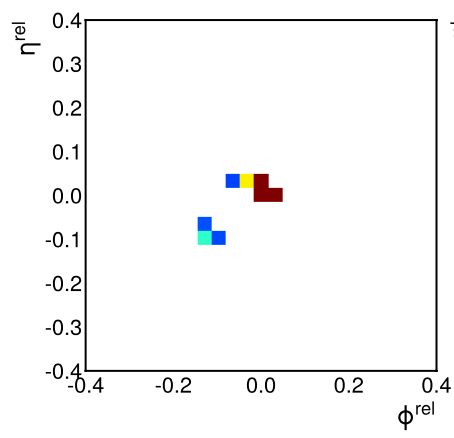
\includegraphics[width=0.3\textwidth]{figures/03-ML/jetimage.png}
    \hspace{0.1\textwidth}
    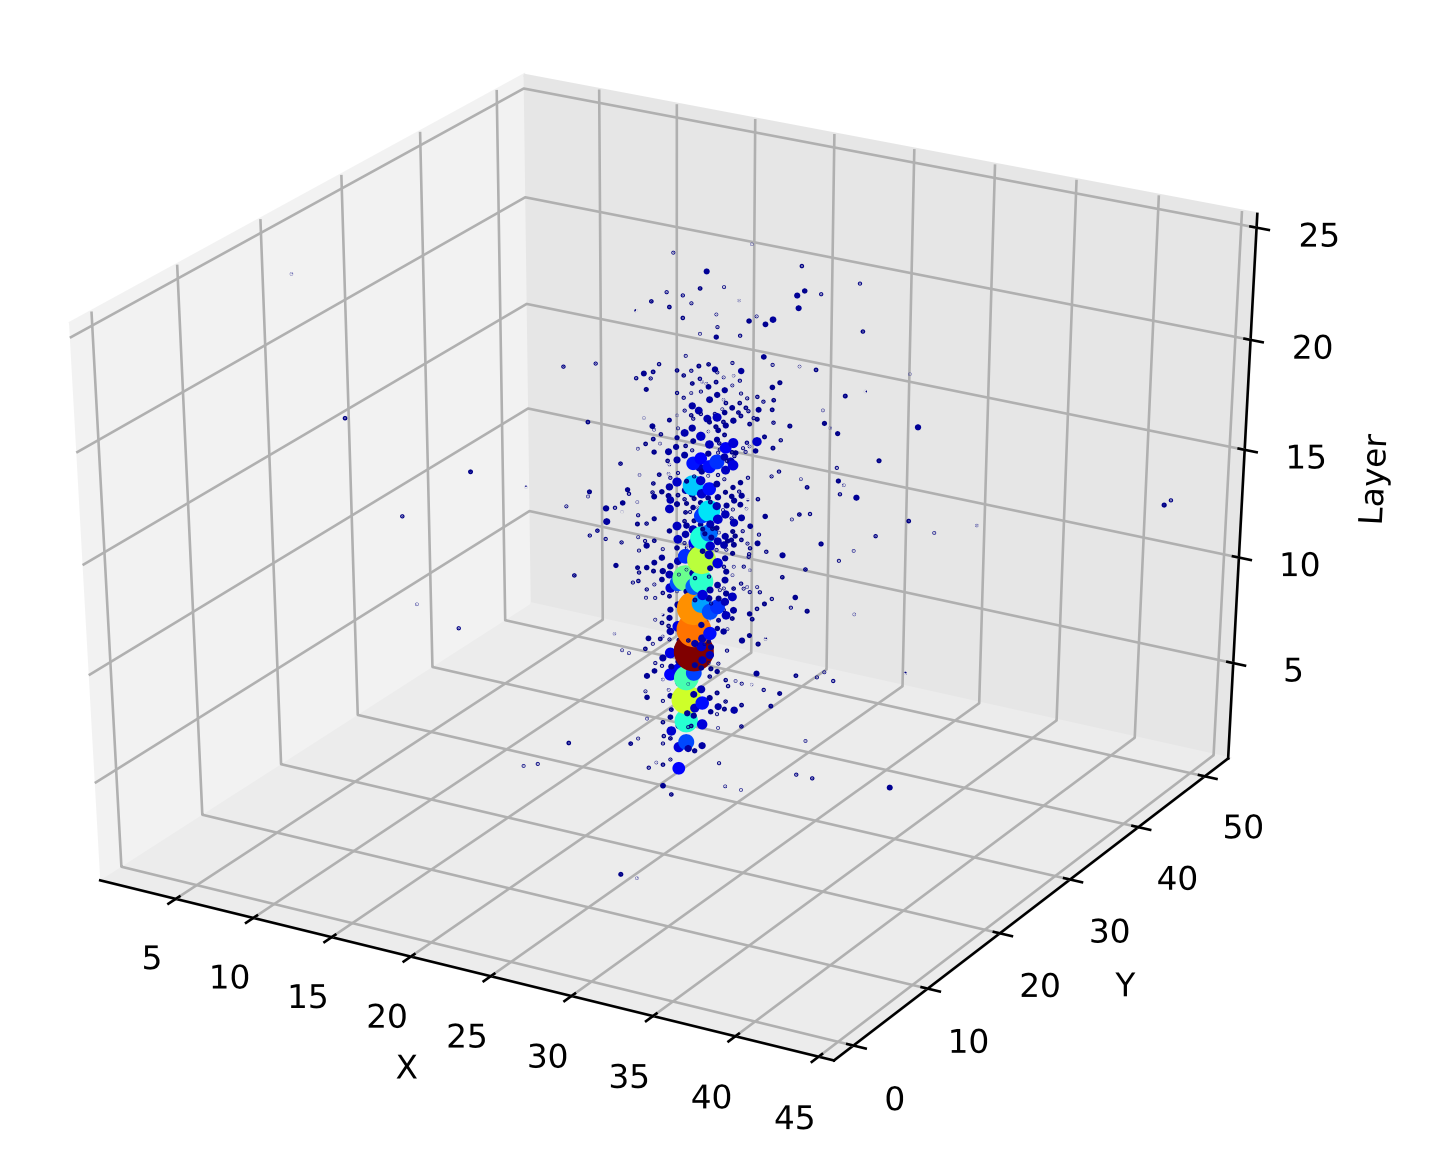
\includegraphics[width=0.38\textwidth]{figures/03-ML/caloimage}
    \caption{Examples of a jet (left) and calorimeter shower (right) represented as 2D and 3D images, respectively.}
    \label{fig:03_ml_jetshowerimage}
\end{figure}

In contrast, GNNs and transformers are naturally: \textit{sparse} --- only the particles or hits need be represented, rather than a dense grid of mostly empty pixels; and \textit{flexible} to the underlying geometry and granularity.
Moreover, they are \textit{permutation invariant} --- learned features are independent of the order of the inputs, which means there is no need to impose an artificial ordering on particles or hits (as opposed to with an MLP, for example).

Finally, in the case of GNNs, the graph topology (i.e. the connections between nodes) can be tuned or even learned to reflect the physical nature of the data.
For example, for local data, such as 3D point clouds of natural objects, connections can be defined based on the Euclidean distance between points, while in the case of jets or particle showers in a calorimeter, we can choose a fully-connected topology to reflect their global correlations (as we emphasize in Chapter~\ref{sec:04_models}).
The attention mechanism in transformers is by definition fully connected, and hence well-suited as well.

This is why we advocate for point-cloud representations and GNN and transformer models as natural choices for HEP data.
Indeed, major contributions of this dissertation are the development of the first point-cloud based generative models for jet simulations (Chapter~\ref{sec:04_models}), which achieve breakthrough performance for an ML simulator in terms of accuracy and efficiency, and the first transformer-based jet tagging algorithm (Chapter~\ref{sec:05_jet_tagging}) for \HVV jet-tagging, powering a significant boost in the sensitivity of the \HH search.
Finally, in Chapter~\ref{sec:06_lgae}, we push the inductive biases of ML models further by incorporating \textit{equivariance} to Lorentz-symmetries, as we introduce next.

\section{Equivariant neural networks}
\label{sec:03_ml_equivariantnns}

ANNs and DL have shown remarkable success in a wide range of computer vision and NLP tasks, motivating applications to the physical sciences.
However, as highlighted in the previous section, the power of DL models is often derived from architectures tuned to the inductive biases of their domains.

A unique feature of physical data is its inherent physical \textit{symmetries} (see Chapter~\ref{sec:01_symmetries}), such as with respect to $\EE[3]$ and Lorentz-transformations for molecules and high-energy collisions, respectively.
It is hence desirable to develop NN architectures that themselves are intrinsically \textit{equivariant} to the associated transformations, which can thereby be more data efficient, more easily interpretable, and perhaps ultimately more successful~\cite{thomas2018tensor}.

We have already encountered some forms of equivariance: to translations in CNNs and to permutations in GNNs.
More recently, there has been work on building equivariance to a broader set of transformations, such as the symmetries mentioned above, which will be the focus of this section.
% We first define equivariance in the context of ML in Section~\ref{sec:06_equivariantnns_equiv}, before discussing three approaches to crafting equivariant NNs in Sections~\ref{sec:06_equivariantnns_e2}---\ref{sec:06_equivariantnns_lorentz}.
% Finally, in Chapter~\ref{sec:06_lgae}, we introduce a novel Lorentz-equivariant ML model for HEP.

\subsection{Equivariance}
\label{sec:06_equivariantnns_equiv}

Let us first introduce precisely what we mean by ``equivariance'', adapting a definition from Refs.~\cite{cohen2016group, cohen2016steerable, worrall2017harmonic, weiler2019general}.

\begin{definition}
\label{def:06_equivariantnns_equiv}
A feature map $f: \CX \rightarrow \CY$ is considered \textbf{equivariant} to a group of transformations $G$ if $\forall g \in G$ and some representation $\pi$ there exists a representation $\pi'$ satisfying
\begin{equation}\label{eq:06_equivariantnns_equiv}
    \pi'(g)f(x) = f(\pi(g)x),
\end{equation}
i.e. the group operation commutes with the map $f$ (and $f$ therefore is an intertwiner).
In this context, $f$ generally represents a NN layer.
Another way to think about this is that each transformation by a group element $g$ on the input must correspond to a transformation by the same group element in the feature space (but with potentially different representations $\pi$ and $\pi'$).
\end{definition}

\begin{definition}
    \textbf{Invariance} is the particular case where $\pi'$ is the trivial representation ($\pi'(g) = \identity$), wherein transformations on $x$ do not affect features at all.
\end{definition}

While for many tasks, such as classification, \textit{invariance} of the outputs is sufficient, Refs.~\cite{worrall2017harmonic, cohen2016steerable} argue that equivariance is more desirable at least in the intermediate layers, as it allows the network to learn useful information about the transformation $g$ itself.

So far, we have discussed CNNs and GNNs / transformers, which are equivariant to the $\mathrm T(N)$ group (translations in $N$ dimensions) and invariant to the $\mathrm S_N$ group (permutations of $N$ objects), respectively.
Next, we discuss the extension to broader symmetry groups.


\subsection{Steerable CNNs for \texorpdfstring{\EE[2]}{E(2)}-equivariance}
\label{sec:06_equivariantnns_e2}

We first describe the generalization of the translational invariance of CNNs to equivariance to not only translations, but \textit{rotations and reflections} in 2D as well; i.e, the $\EE[2]$ group.
We make use of a general procedure, based on Refs.~\cite{cohen2016group, cohen2016steerable}, for extending 2D translational invariance ($\mathrm T(2)$) to equivariance to a group $G =  \mathrm T(2)\rtimes H$, where $\rtimes$ is the semi-direct product and $H$ is a subgroup of $G$, meaning we can induce representations of $G$, $\mathrm{Ind}^G_H$, from $H$.\footnote{See e.g. Chapter IV, p297 of Ref.~\cite{Zee:2016fuk} for induced representations of \EE[2].}
For $G = \EE[2]$, in particular, $H = \mathrm O(2)$, the group of distance-preserving transformations in 2D; i.e., rotations and reflections.

The key idea in developing a $G$-equivariant layer is to first find the set of maps $F \ni f$ which satisfy Eq.~\ref{eq:06_equivariantnns_equiv} for an element $h \in H$:
\begin{equation}\label{eq:06_equivariantnns_equiv2}
    \ro(h)f = f\ri(h)
\end{equation}
where $\ro$ and $\ri$ are reps of $H$. After this, Eq.~\ref{eq:06_equivariantnns_equiv} can be automatically satisfied using
\begin{equation}
    \pi'(g)f = \mathrm{Ind}^G_H(g)f = \ro(h)f(\ri(h^{-1})(x-t))
\end{equation}
where $g = th$ for some 2D translation $t \in \mathrm T(2)$.

% One simple method for finding $F$ is to recognize that since Eq.~\ref{eq:06_equivariantnns_equiv2}
Since Eq.~\ref{eq:06_equivariantnns_equiv2} is linear in $f$, we want a complete linear basis of functions that satisfy it.
We can obtain this by restricting the convolutional filters of a standard CNN to circular harmonics~\cite{worrall2017harmonic}:\footnote{See Refs.~\cite{weiler20183d, weiler2019general} for a more rigorous derivation.}
\begin{equation}\label{eq:06_equivariantnns_circharms}
    W_m(r, \phi; R, \beta)=R(r)e^{i(m\phi + \beta)},
\end{equation}
where the radial component $R$ and the filter phase $\beta$ are learnable parameters.
We can see that $m \in \mathbb Z$, these filters form a complete basis and satisfy Eq.~\ref{eq:06_equivariantnns_equiv2} under convolutions ($*$) with an image $F(r, \phi)$ rotated by $\theta$:
\begin{equation}
    W_m * F(r, \phi + \theta) = e^{im\theta} W_m * F(r, \phi).
\end{equation}
Here we took $\ri$ to be the fundamental $\SO[2]$ rep acting on the image and $\ro$ to be any one of the infinite complex reps.
After discretizing these filters Ref.~\cite{worrall2017harmonic} demonstrates significant improvement in classification of rotated images compared to SOTA CNNs.
Such networks are generally referred to as ``Steerable CNNs'', and, in practice, are implemented using a finite set of $N$ such circular harmonic filters, with $m \in \{0, \frac{2\pi}{N}, ..., \frac{2\pi(N-1)}{N}\}$ (and possibly their reflections), which are then pooled in a rotationally-invariant manner, as illustrated in Figure~\ref{fig:06_equivariantnns_scnn}.

\begin{figure}[ht]
    \centering
    \captionsetup{justification=centering}
    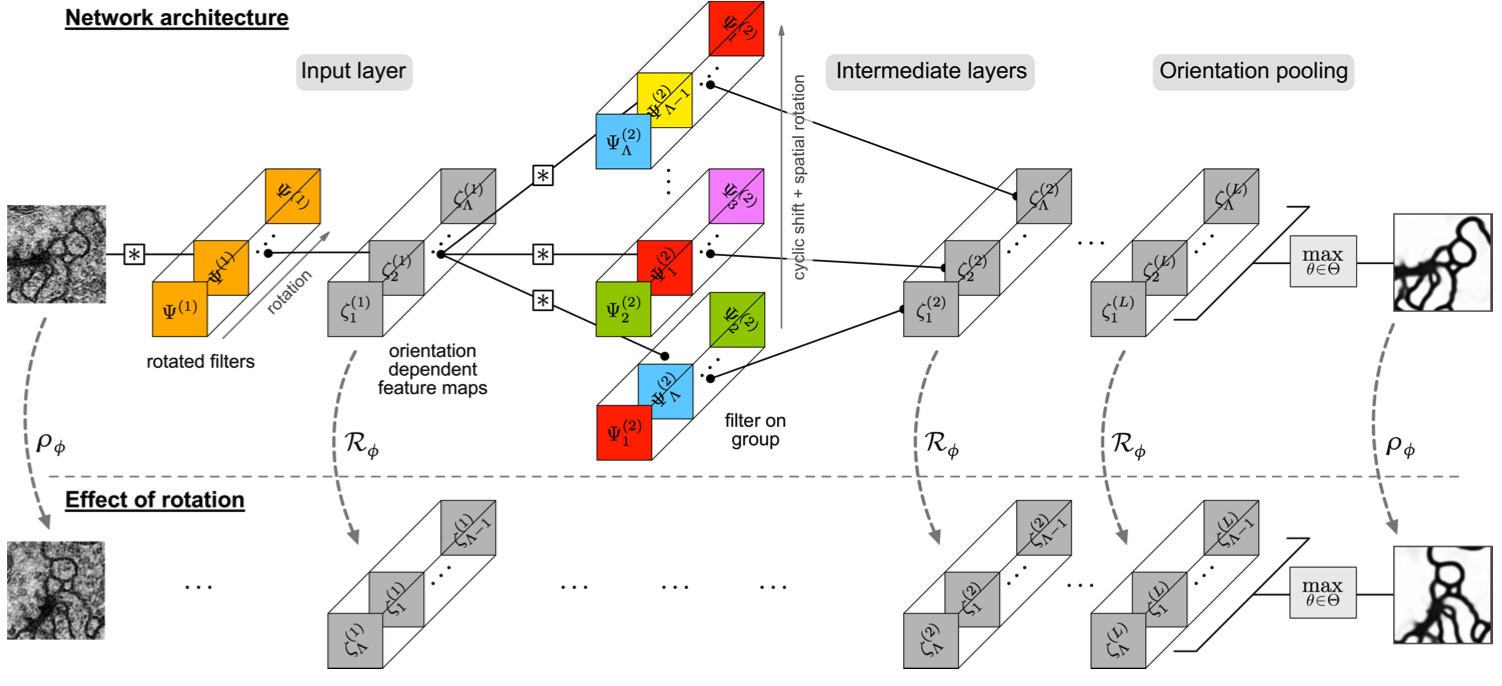
\includegraphics[width=\textwidth]{figures/06-ML4Jets/equivariantnns/scnns}
    \caption{Schematic of a steerable CNN, reproduced from Ref.~\cite{weiler2018learning}.}
    \label{fig:06_equivariantnns_scnn}
\end{figure}


\subsection{Tensor-field networks for \texorpdfstring{\EE[3]}{E(3)}-equivariance}
\label{sec:06_equivariantnns_e3}

Steerable CNNs have been extended to $\EE[3]$-equivariance --- translations, rotations, and reflections in 3D --- as well~\cite{weiler20183d}.
However, we will discuss a slightly different approach, applied to point-cloud data.
This approach uses ``Fourier decompositions'' of the input, feature, and output spaces into irreducible representations (irreps) of the symmetry group, and is referred to as a ``tensor-field network''~\cite{thomas2018tensor}.
In addition to their aforementioned applications to HEP, point clouds are also extremely useful representations of physical objects such as molecules and crystals, both of which are inherently $\EE[3]$ invariant.

In the approach of Ref.~\cite{thomas2018tensor}, the input and intermediate network layers $f$ take the set of coordinates $\cvec{r}_a$ and features $\cvec{x}_a$ for each point $a$ in the point cloud and map them to the same set of coordinates with new learned features $\cvec{y}_a$ ($f(\cvec{r}_a,\cvec{x}_a) = (\cvec{r}_a,\cvec{y}_a)$), with an equivariant $f$ again having to satisfy Eq.~\ref{eq:06_equivariantnns_equiv}.
If necessary, the features are aggregated at the end across all points to produce the output.
Translation equivariance is achieved directly by requiring $f$ to only consider distances $\cvec{r}_i - \cvec{r_j}$ between points $i$ and $j$ (a global translation will not affect these).

For rotation equivariance, first the feature vectors $\cvec{x}_a$ are decomposed according to how they transform under irreps of $\SO[3]$ --- scalars, vectors or higher order tensors (the coordinates $\cvec{r}_a$ already transform as vectors in $\mathbb R^3$ under the fundamental rep):
\begin{equation}
    \mathbb R^3 \oplus \CX = \bigoplus _l R_l^{m_l}
\end{equation}
where the sum is performed over irreps $R_l$ (with dimension $2l+1$) and $m_l$ are the multiplicities.
Thus, each point's features and coordinates have the corresponding decomposition:
\begin{equation}
    \cvec{r}_a \oplus \cvec{x}_a = \bigoplus _l \bigoplus _{c=1}^{m_l} V^l_{ac}
\end{equation}
where the $V^l_{ac}$ are tensors which transform under the $l$ irrep.
Similar to steerable CNNs, each of these tensors are individually acted upon by generalized convolutional filters with the form $R(r)Y^{l_f}(\hat{r})$, where $R$ is a learned radial function, $Y^l$ are the spherical harmonic tensors, and the set $l_f$ corresponds to the set of desired irreps in feature space. The spherical harmonics are directly analogous to using circular harmonics for $\EE[2]$ (except they have dimension $2l+1$) and by the same argument they satisfy Eq.~\ref{eq:06_equivariantnns_equiv}.
This convolution effectively produces a tensor product representation of $\SO[3]$ $R_{l} \otimes R_{l_f}$, which is then decomposed via Clebsch-Gordan (CG) decomposition into irreps again.

A useful pedagogical example is of a network taking as input a collection of point masses and outputting the inertia tensor.
The input features are the masses of each point, which are scalars under $\SO[3]$, and the inertia tensor transforms as the $0 \oplus 2$ representation, so we define this network to be of the type $0 \rightarrow 0 \oplus 2$.

Some interesting and successful applications include classifying molecules~\cite{miller2020relevance}, predicting protein complex structures~\cite{Eismann2020HierarchicalRN}, and predicting the phonon density of states (DoS) in crystals~\cite{chen2020direct}.
A schematic of the architecture used for the latter is shown in Figure~\ref{fig:06_equivariantnns_dos}.
Different crystals are represented geometrically as point clouds in $\mathbb R^3$, with individual atoms labeled via feature vectors $\cvec{x}_a$ using mass weighted one-hot encoding.
After a series of convolution layers the features are summed over all points to predict 51 scalars comprising the phonon DoS.


\begin{figure}[ht]
    \centering
    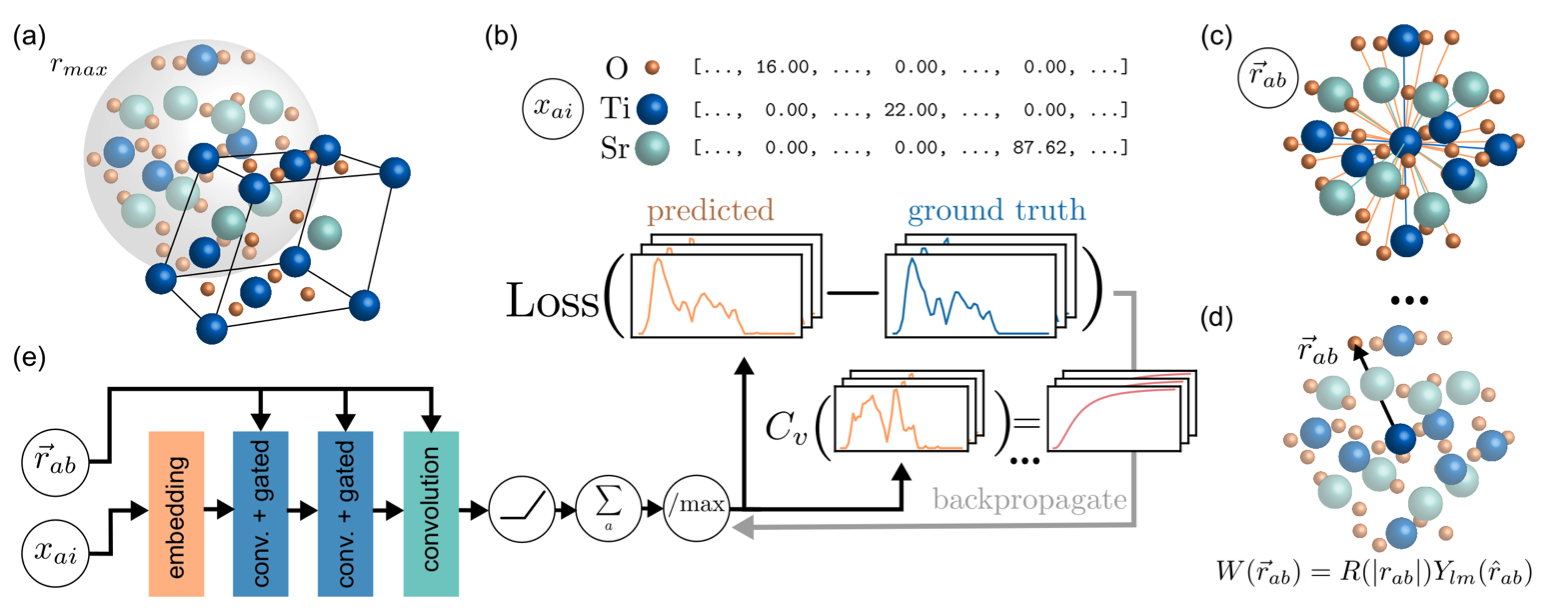
\includegraphics[width=\textwidth]{figures/06-ML4Jets/equivariantnns/dos}
    \caption{Schematic of the $\EE[3]$-equivariant neural network architecture used for predicting phonon density of states, reproduced from Ref.~\cite{chen2020direct}.}
    \label{fig:06_equivariantnns_dos}
\end{figure}


\subsection{Lorentz-group-equivariant networks}
\label{sec:06_equivariantnns_lorentz}

Recently there has been some success in creating Lorentz-group-equivariant networks, which are desirable for DL applications to high energy data.
The Lorentz group $\mathrm{O}(3, 1)$ comprises the set of linear transformations between inertial frames with coincident origins.
Henceforth, we restrict ourselves to the special orthochronous Lorentz group $\mathrm{SO}^+(3, 1)$, which consists of all Lorentz transformations that preserve the orientation and direction of time.
Equivariance to such transformations is a fundamental symmetry of the data collected out of high-energy particle collisions.

To our knowledge, there has been no generalization of steerable CNNs to the Lorentz group; however, Refs.~\cite{equivariance-Fourier-Kondor,equivariance-Fourier-Anderson,E(2)-Equivariant, bogatskiy2020lorentz} propose an alternative, completely Fourier-based approach, again acting on point clouds, that shares some similarities with the $\EE[3]$-equivariant network discussed above.

The general method is to:

\begin{enumerate}
    \item Decompose the input space into irreps of the group.
    \item Apply an equivariant mapping (satisfying Eq.~\ref{eq:06_equivariantnns_equiv}) to the feature space.
    \item Take tensor products of the irreps and CG-decompose them again into irreps.
    \item Repeat steps 2--3 until the output layer.
\end{enumerate}

The crucial difference between this and the previous networks is that the mapping is no longer via convolutional filters; instead, it is chosen to be a simple linear aggregation across the nodes of the point clouds.
Recall from Definition~\ref{def:06_equivariantnns_equiv} that equivariant maps $f$ must be intertwiners between input and output representations, which, according to Schur's Lemma, imposes strong restrictions on both the form of a linear $f$ and its output $f(x)$. Namely: the outputs and inputs must have the same irrep decomposition (though the multiplicities are allowed to vary, akin to increasing/decreasing the ``channels'' in an image) and $f$ must be a direct sum of learned matrices acting individually on each irrep. The transformation between $f^{\mathrm{in}}$ and $f^{\mathrm{pre}}$ in Figure~\ref{fig:06_equivariantnns_equivneuron} illustrates such a mapping.

\begin{figure}[t]
    \centering
    % \captionsetup{justification=centering}
    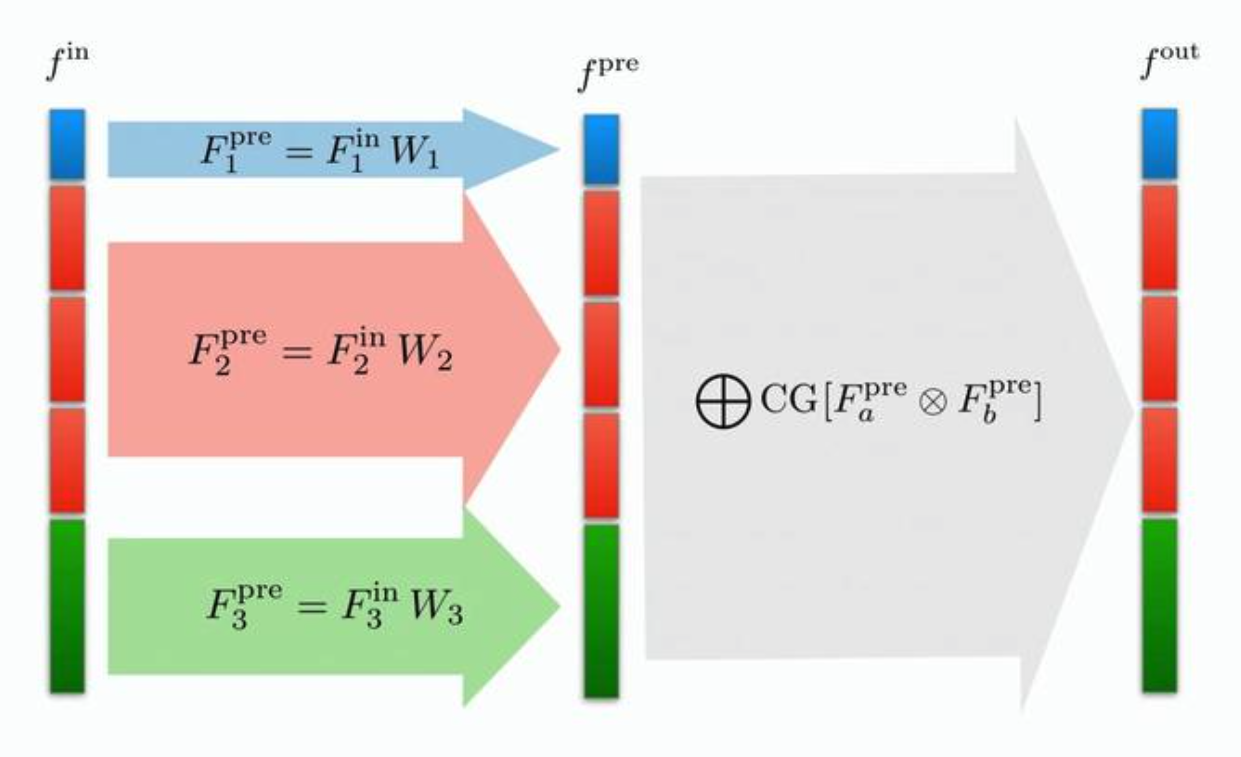
\includegraphics[width=0.7\textwidth]{figures/06-ML4Jets/equivariantnns/equivneuron}
    \caption{Schematic of a Lorentz group-equivariant network layer, reproduced from Ref.~\cite{bogatskiy2020lorentz}.}
    \label{fig:06_equivariantnns_equivneuron}
\end{figure}

% Since this mapping is now linear, we need another way of injecting group equivariant non-linearities into the network.
To inject non-linearities into the network, Ref.~\cite{bogatskiy2020lorentz} proposes to take tensor products between each pair of irreps after the mapping, and then perform a CG decomposition.\footnote{See Ref.~\cite{gelfand2018representations} for a detailed analysis of CG decomposition for the Lorentz group.}
Another freedom available to us is acting with arbitrary learned functions on any scalar irreps that result from the decomposition, since they are, by definition, Lorentz-invariants.

One successful application of this network has been to jet tagging:
Ref.~\cite{bogatskiy2020lorentz} successfully applied this ``Lorentz-group network'' (LGN) to top-quark identification, demonstrating a high (92.9\%) accuracy, though they were unable to match the then-SOTA (93.8\% using the ParticleNet GNN~\cite{Qu:2019gqs}).

Finally, we note that overall this is, in fact, a very general approach: applicable to any symmetry group.
This includes the aforementioned $\EE[2]$ and $\EE[3]$ groups as well as potentially more exotic groups such as $E_8$ or $G_2$ which also arise in physics.
The only group-dependent operations in such a network are the decompositions into irreps which can readily be calculated for any group (as opposed to steerable CNNs where one needs to derive group equivariant kernels/convolutional filters).

\subsubsection{Summary}
\label{sec:06_equivariantnns_conclusion}

We reviewed three approaches to creating neural networks that are equivariant to physical symmetry groups: by extending the translation-equivariant convolutions in CNNs to more general symmetries with appropriately defined learnable filters as in Refs.~\cite{equivariance-kernel-Cohen,equivariance-kernel-Finzi,cohen2016group}, by operating in the Fourier space of the group~\cite{bogatskiy2020lorentz}, and a combination thereof~\cite{thomas2018tensor}.
Such networks are highly relevant to the physical sciences, where datasets often possess intrinsic symmetries, and, as demonstrated in some example tasks, they are promising alternatives and improvements to standard non-equivariant DL approaches.
In particular, Lorentz-equivariant networks have shown promise in jet classification, a key task in HEP.
In Chapter~\ref{sec:06_lgae}, we will discuss the extension of these ideas to the first Lorentz-equivariant \textit{autoencoder} for jets, with applications to data compression, anomaly detection, and potentially fast simulations as well.


\section{Autoencoders and generative models}
\label{sec:03_genaes}

\subsection{Autoencoders and anomaly detection}
\label{sec:03_aes}

\begin{figure}[ht]
    \centering
    \captionsetup{justification=centering}
    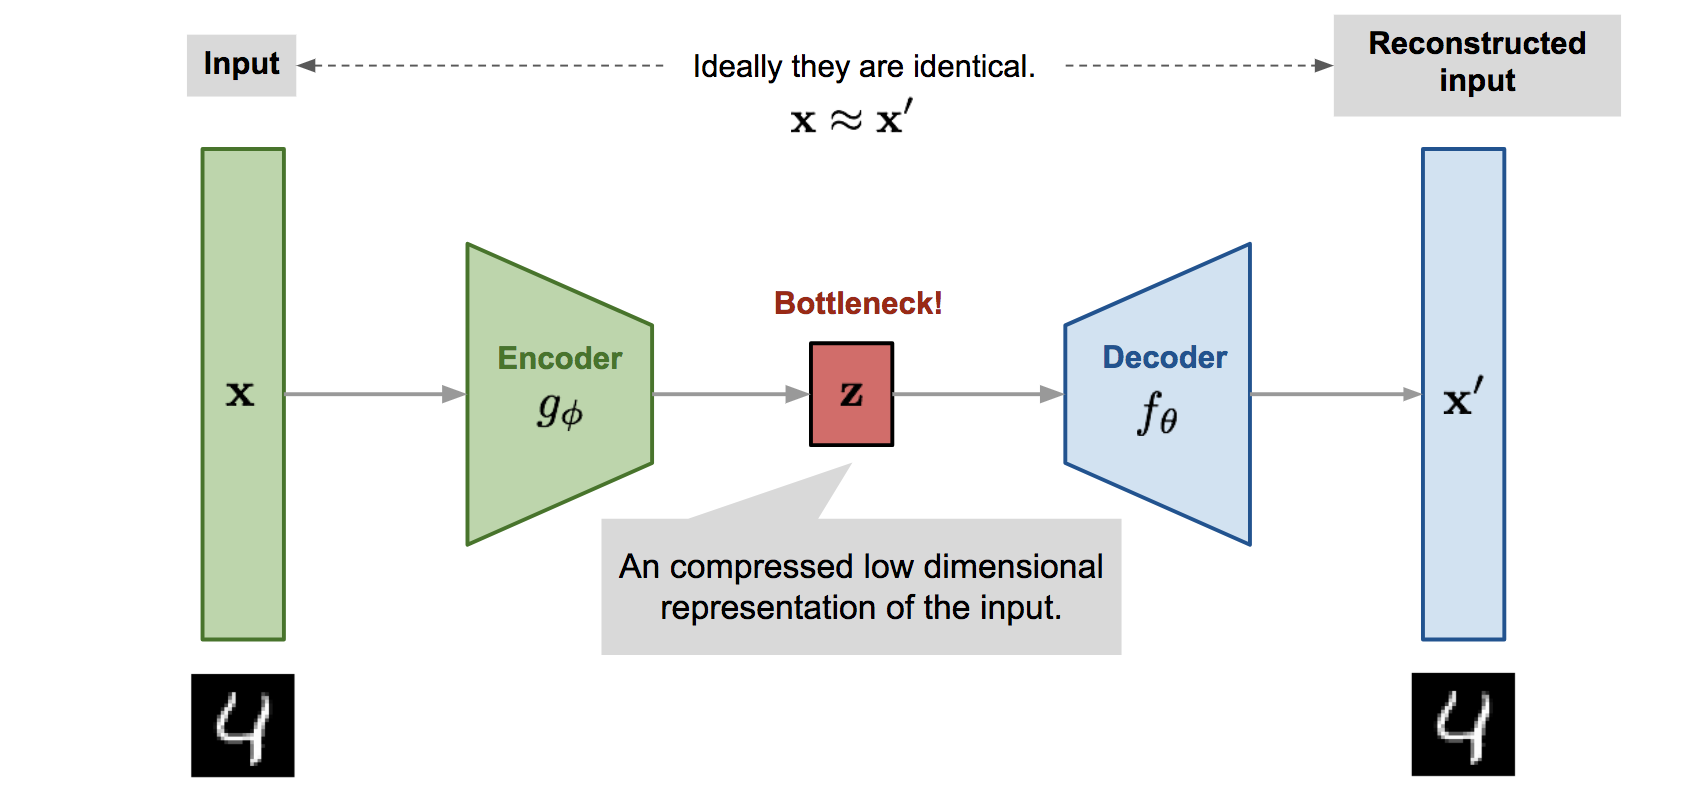
\includegraphics[width=\textwidth]{figures/03-ML/autoencoder-architecture.png}
    \caption{Diagram of an image autoencoder, reproduced from Ref.~\cite{weng2018VAE}.}
    \label{fig:03_ml_autoencoder}
\end{figure}

In this final section, we discuss two paradigms of unsupervised learning relevant to this dissertation: autoencoders (AEs) and generative models.
AEs are NN architectures composed of an \textit{encoder} network, which maps the input into a typically lower dimensional latent space --- called a ``bottleneck'' --- and a \textit{decoder}, which attempts to reconstruct the original input from the latent features (Figure~\ref{fig:03_ml_autoencoder}).
The bottleneck encourages AEs to learn a compressed representation of data that captures salient properties~\cite{autoencoders}, which can be valuable in HEP for compressing the significant volumes of data collected at the LHC~\cite{Guglielmo}.

The learned representation can also be exploited for later downstream tasks, such as anomaly detection, where an autoencoder is trained to reconstruct data considered ``background'' to our signal, with the expectation that it will reconstruct the signal worse than the background.
Thus, examining the reconstruction loss of a trained autoencoder may allow the identification of anomalous data.
This can be an advantage in searches for new physics, since instead of having to specify a particular signal hypothesis, a broader search can be performed for data incompatible with the background.
This approach has been successfully demonstrated in Refs.~\cite{Heimel:2018mkt,Farina-anomaly,Cerri:2018anq,Finke-anomaly,Kasieczka:2021xcg,Govorkova:2021utb,Pol:2020weg,Ngairangbam:2021yma,Dillon-lower-dimension}.
Two recent exciting examples from CMS include a model-agnostic search for di-jet resonances with Run 2 data~\cite{CMS-PAS-EXO-22-026}, which prominently uses AEs for multiple search strategies, and a new AE-based online Level-1 trigger paths implemented in Run 3~\cite{CMS-DP-2023-079, CMS-DP-2024-059}.

Furthermore, there are many possible variations to the general autoencoder framework for alternative tasks~\cite{AE-review-1,AE-review-2}, such as variational autoencoders (VAEs)~\cite{VAE}, which we discuss in the next section.
While there have been some recent efforts at GNN-based autoencoder models~\cite{Tsan:2021brw,Atkinson:2021nlt}, in this dissertation, we present the first Lorentz-equivariant autoencoder for jets in Chapter~\ref{sec:06_lgae}.
We focus on data compression and anomaly detection but note that our model can be extended to further applications, such as fast simulations in HEP.

\subsection{Generative models}
\label{sec:03_generative}

\begin{figure}[ht]
    \centering
    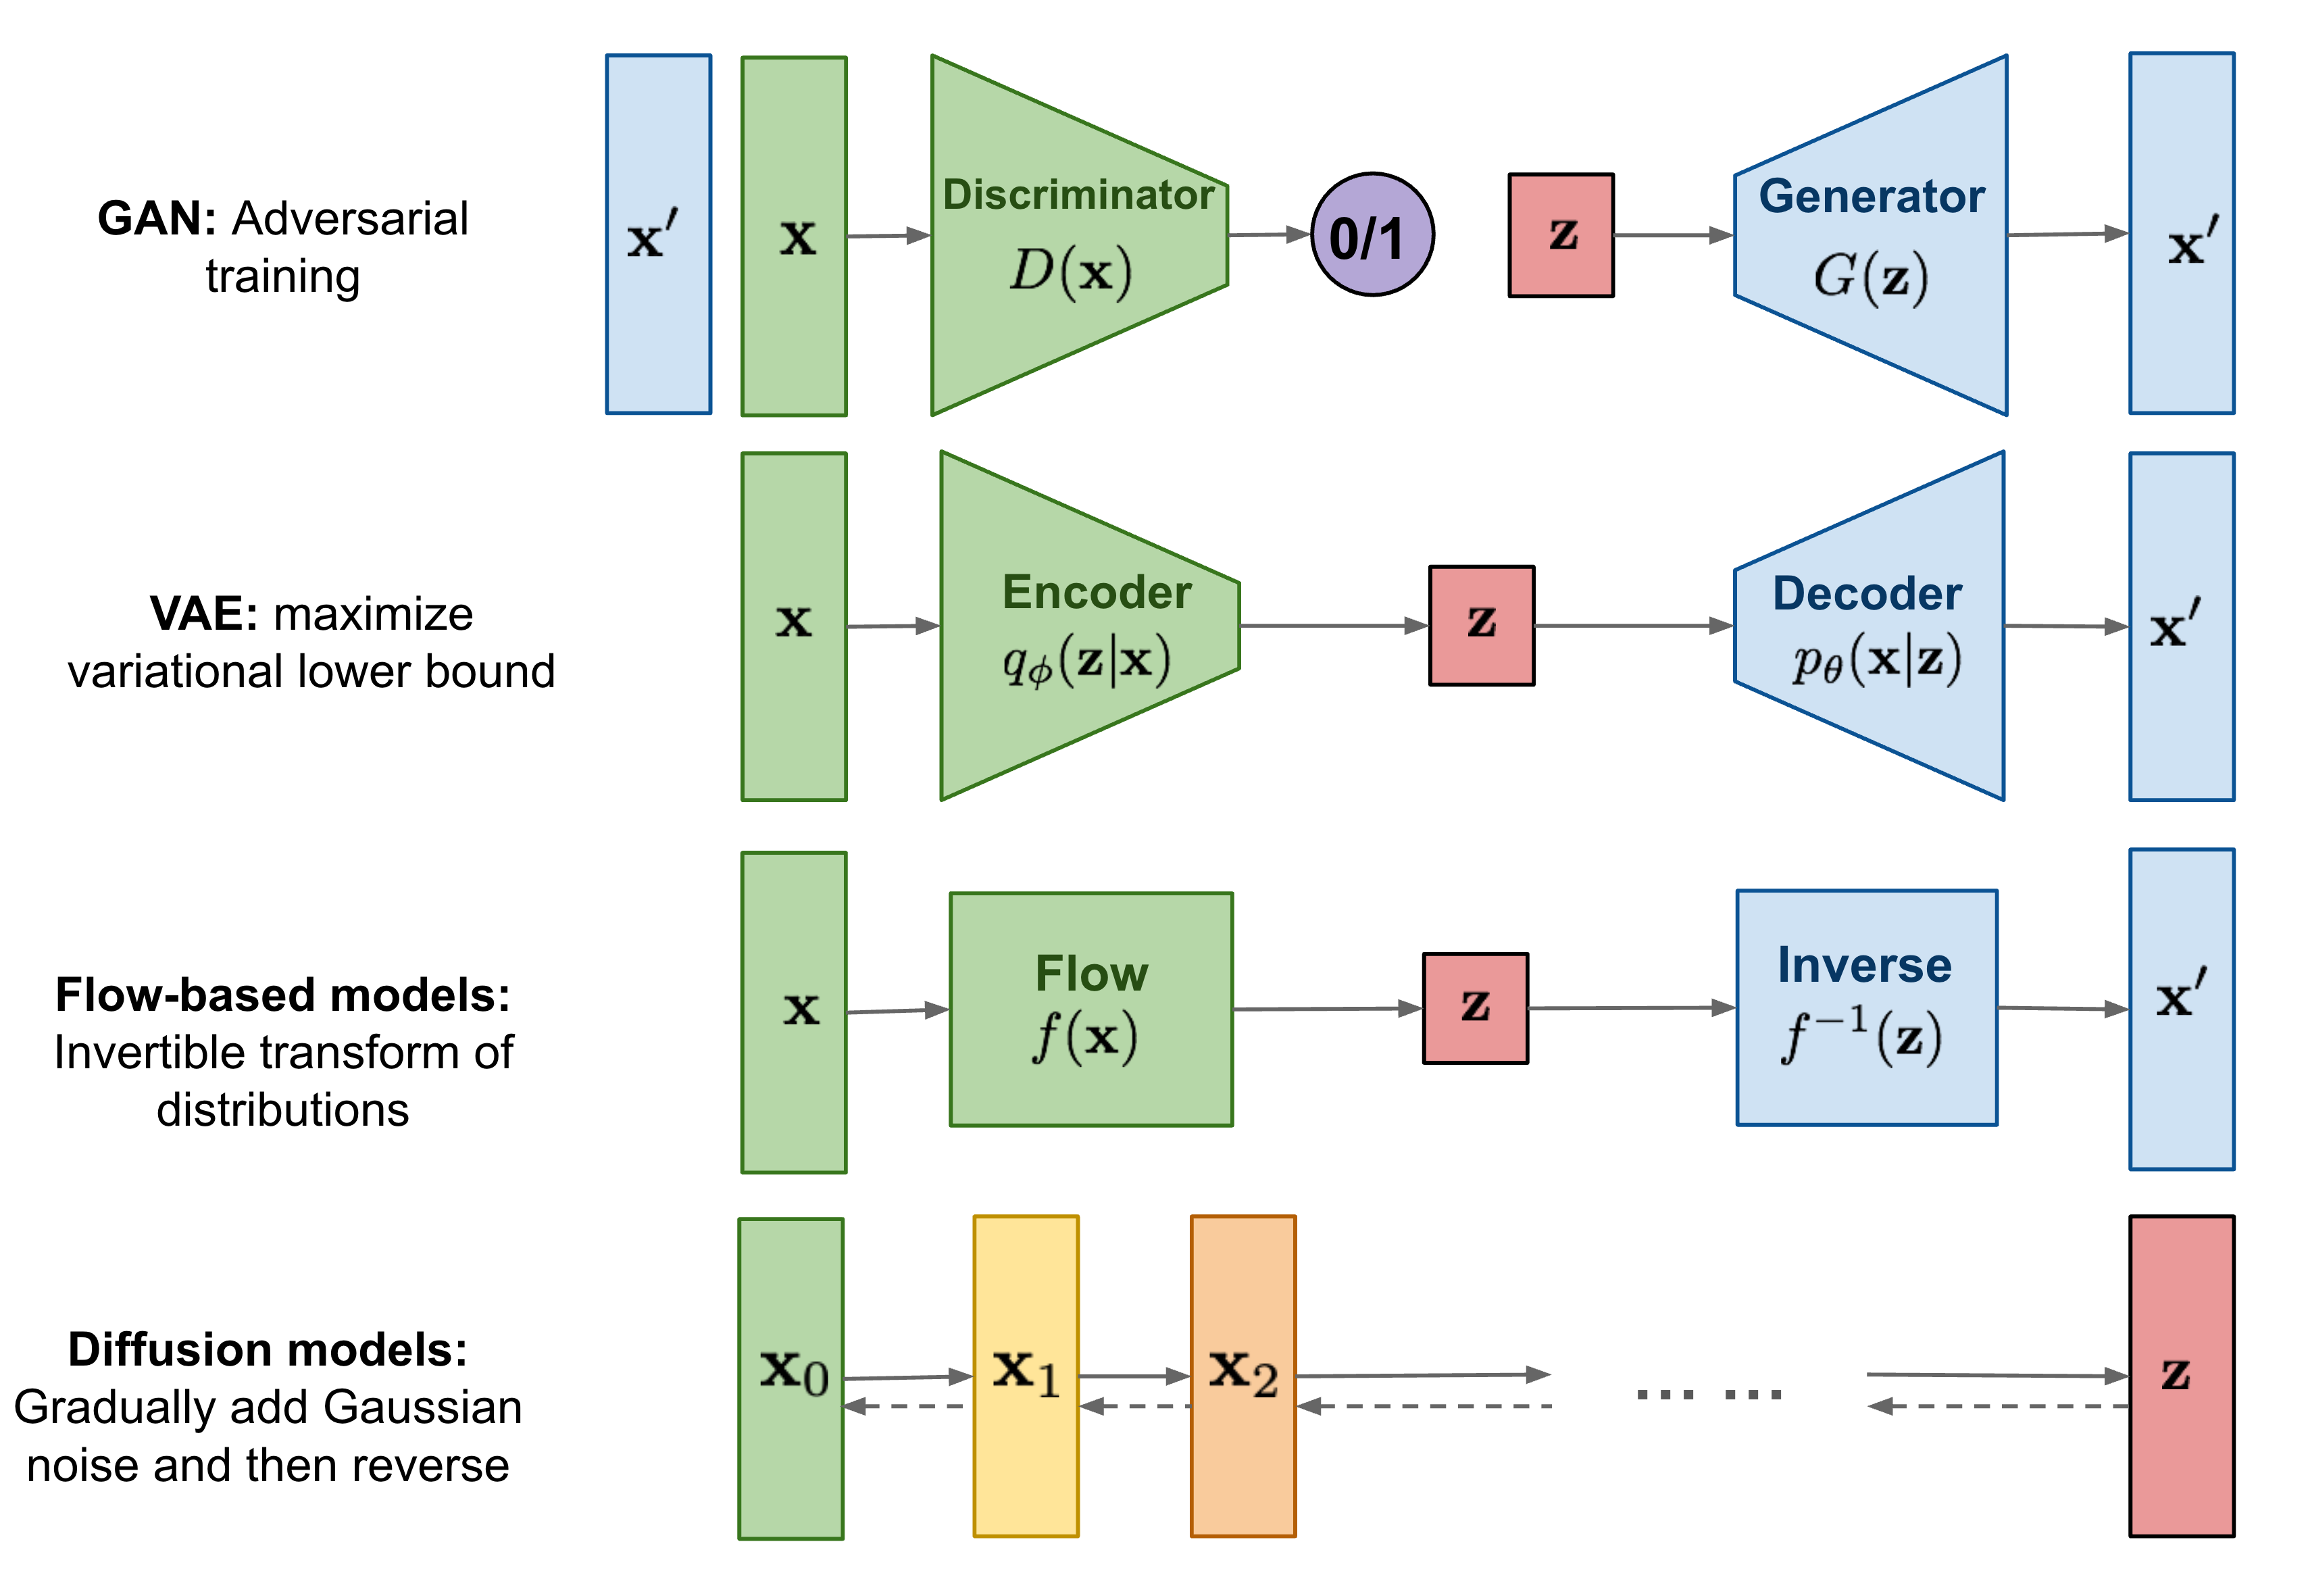
\includegraphics[width=\textwidth]{figures/03-ML/generative-overview.png}
    \caption{Summary of popular generative models, reproduced from Ref.~\cite{weng2021diffusion}.}
    \label{fig:03_ml_generative}
\end{figure}

Generative models are a class of statistical models that aim to capture the probability distribution of the data $p(x)$ in order to generate new samples.
This is a challenging problem, but one that has seen significant progress in recent years with DL, particularly in computer vision and NLP.
We will briefly walk through four popular approaches, illustrated in Figure~\ref{fig:03_ml_generative}, which can be broadly categorized as \textit{likelihood-based} or \textit{implicit} models.

\subsubsection{Likelihood-based models}

Likelihood-based models attempt to directly learn the probability distribution of the data through some form of (approximate) likelihood maximization.\footnote{See the next chapter for an introduction to likelihoods.}
Flow-based models, for example, learn a series of invertible transformations to map a simple base distribution that is easy to sample from, such as a Gaussian, to the complex target data distribution.
The most popular of these at the time of writing are ``normalizing flows'', which require each transformation to have a tractable Jacobian determinant with which to correctly normalize the result.
% Normalizing flows have been applied to a wide range of tasks, including image~\cite{NICE,RealNVP,Glow} and calorimeter shower generation~\cite{ATL-SOFT-PUB-2018-001}.

Normalizing flows have a number of advantages, such as their simple and intuitive training objective --- maximizing the likelihood of each data point --- and a tractable likelihood evaluation.
These have led to successful applications to density estimation and generation tasks in both computer vision~\cite{dinh2017density, kingma2018glow} and HEP~\cite{Krause:2021ilc}.
However, the constraint of invertible transformations with tractable Jacobians turns out to be extremely restrictive on the model design and expressivity in practice~\cite{fjelde2024flow, hawley2024flow}, generally resulting in worse performance on high-dimensional data compared to the models we discuss below.
Recently, over the last year, a related (in spirit) class of models without the normalization constraint, called ``flow-matching'' models, have emerged with extremely promising and, in some cases, state-of-the-art (SOTA) results on images~\cite{liu2023flow, lee2024improving}.

Another example of a likelihood-based model is the variational autoencoder (VAE)~\cite{VAE}, which is structurally similar to an AE in that it has an encoder mapping an input data point into a latent representation, and a decoder mapped that back to the original.
They key novelty, however, is that the latent space is encouraged through the loss function to follow a well-defined simple distribution to sample from --- again, typically, a Gaussian.
Explicitly, the VAE loss function is a combination of the reconstruction loss of a standard AE and the Kullback-Leibler divergence between the learned latent distribution and the assumed prior.
Together, this can be shown to approximate the evidence lower bound (ELBO) of the true likelihood~\cite{VAE}, which is why VAEs are thought of as likelihood-based.

VAEs were one of the early success stories in generative modeling, with a relatively simple implementation, training, and learning objective.
However, they again are restrictive, this time due to the strong assumption imposed on the latent space, which actually competes with the reconstruction objective, and which, if incorrect, limits the performance.
Indeed, our early studies in HEP showed that the learned latent space of VAEs is manifestly non-Gaussian for jets, leading to suboptimal performance with a Gaussian latent prior~\cite{Orzari_2023}.
This is why VAEs also generally yield poorer performance than \textit{generative adversarial networks} (GANs)~\cite{Goodfellow:2014upx}, which we discuss next.

\subsubsection{GANs}

GANs are a type of implicit generative model.
This means they learn to generate samples without directly learning the likelihood of the data.
Instead, their loss function is effectively provided by a second neural network, called the discriminator or critic, which tries to distinguish between real and generated samples.
The two generator and discriminator networks, with the former aiming to fool the latter, are trained iteratively and \textit{adversarially}, forming a feedback loop and progressively improving each other.
This continues until, ideally, the duo converge to a point where the generator produces samples indistinguishable from the real by the discriminator.

GANs have an interesting game-theoretic interpretation as a minimax game, where the Nash equilibrium, or global optimum, is achieved through minimizing the Jensen-Shannon divergence between the real and generated data distributions~\cite{Goodfellow:2014upx}.
Several variations of GANs have also been proposed, including the Wasserstein-GAN~\cite{arjovsky2017wasserstein}, which instead aims to minimize the Wasserstein distance between the two distributions.

Due to the adversarial nature of the training, GANs are notoriously difficult to train~\cite{salimans2016improved, arjovsky2017towards, arjovsky2017wasserstein, mescheder2018training}.
However, their formulation poses no restrictions on the form of the generator while providing a powerful loss function and feedback mechanism.
When trained successfully, this leads to expressive, flexible, and extremely successful generative models in a wide variety of domains.
Indeed, at the time of the work of this dissertation, GANs were the SOTA in computer vision~\cite{karras2019style, brock2019large, karras2020analyzing} and had shown promising signs in HEP as well~\cite{deOliveira:2017pjk, Paganini:2017dwg, ATL-SOFT-PUB-2018-001, ATL-SOFT-PUB-2020-006, Erdmann:2018jxd, Carminati:2020kym}.
However, as we highlight below, there had been no successful application of GANs, or indeed any generative model, to point cloud data and GNNs or transformers in HEP.

\subsubsection{Score-based diffusion models}

Finally, we briefly note the recent development in the past two years of a new class of generative models, called \textit{diffusion} or \textit{score-based} models~\cite{ho2020denoising, song2021score}.
These models iteratively ``denoise'' initial Gaussian noise into something resembling samples from the true data distribution; conceptually, this is related to diffusion in physical systems.
The breakthrough with these models came from recognizing that, with the right learning objective, this denoising process is in fact equivalent to following the gradient of the log-likelihood function, AKA the \textit{score}.

Diffusion models allow a likelihood-driven training objective, like flow-based models, but without the restrictive constraints (as the score does not need to be normalized!), thereby offering the flexibility of a GAN along with a far more stable training procedure.
This, combined with several innovations in training and inference techniques, has led to diffusion models surpassing GANs in computer vision~\cite{dhariwal2021diffusion}, and showing promising signs over the last year in HEP as well (in part enabled by the work in this dissertation, as we discuss in Chapter~\ref{sec:04_outlook}).
However, so far, diffusion models remain computationally expensive, with inference naively requiring up to hundreds of denoising steps, which limits their application to fast simulations.
Nevertheless, they are an exciting area for exploration in future work.

\subsection{Previous work}
\label{sec:04_mpgan_genhep}

\textit{Note: the following discussion represents the state of the field at the time of our first publications in 2021, to provide context.
Since then, the field has evolved significantly, partly due to the work presented in this dissertation, as we discuss in Chapter~\ref{sec:04_outlook}.
}

\subsubsection{Generative modeling in HEP}

Past work in generative modeling in HEP exclusively used image-based representations for HEP data.
The benefit of images is the ability to employ CNN-based generative models, which have been highly successful on computer vision tasks.
References~\cite{deOliveira:2017pjk, Paganini:2017dwg, ATL-SOFT-PUB-2018-001, ATL-SOFT-PUB-2020-006, Erdmann:2018jxd, Carminati:2020kym},
for example, build upon CNN-based GANs, and Ref.~\cite{sarm} uses an autoregressive model, to output jet- and detector-data-images.

However, as highlighted in Section~\ref{sec:03_ml_physics}, the high sparsity of the images can lead to training difficulties in GANs, while the irregular geometry of the data poses a challenge for CNNs which require uniform matrices.
While these challenges can be mitigated to an extent with techniques such as batch normalization~\cite{ioffe2015batch} and using larger/more regular pixels~\cite{ATL-SOFT-PUB-2020-006}, the approach we develop avoids both issues by generating particle-cloud-representations of the data, which are inherently sparse data structures and completely flexible to the underlying geometry.


\subsubsection{Point cloud generative modeling}
\label{sec:04_mpgan_pcgans}

% In the context of ML, jets can be represented in multiple ways.
% Two more spatially efficient representations are as ordered lists or unordered sets~\cite{Shlomi:2020gdn,Duarte:2020ngm} of the jet constituents and their features.
% The difficulty with the former is that there is no particular preferred ordering of the particles---one would have to impose an arbitrary ordering such as by transverse momentum~\cite{Sirunyan:2020lcu}.
% The more natural representation is the unordered set of particles in momentum space, which we refer to as a ``particle cloud.''

\begin{figure}[ht]
    \centering
    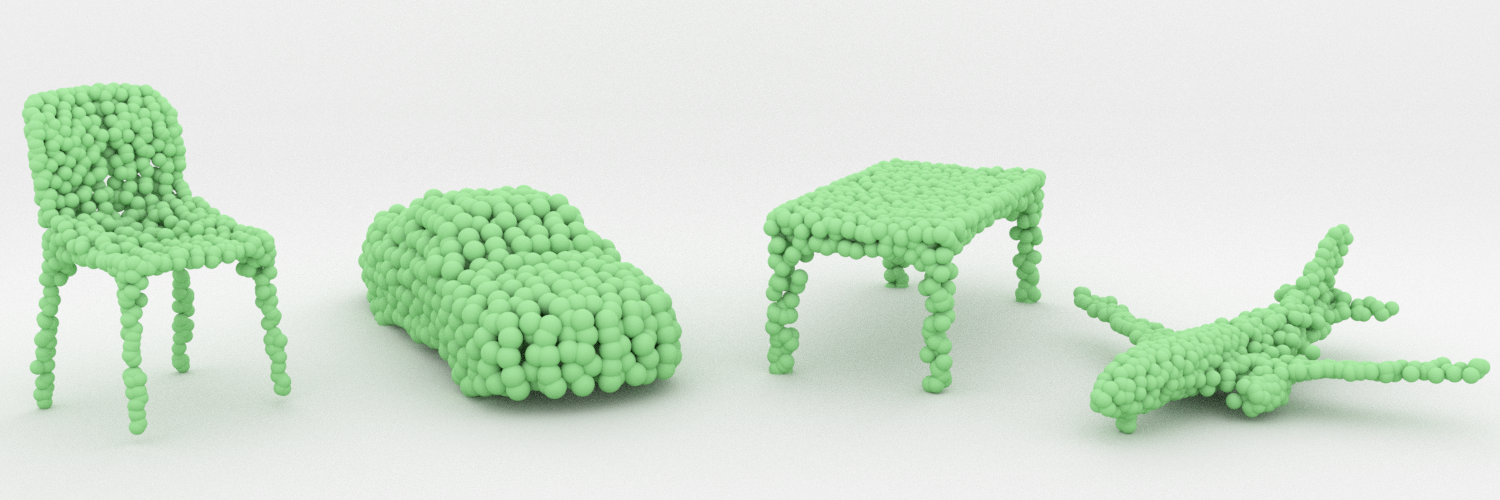
\includegraphics[width=\textwidth]{figures/03-ML/shapenet}
    \caption{Sample point clouds from the ShapeNet dataset, reproduced from Ref.~\cite{DBLP:journals/corr/GadelhaMW17}.}
    \label{fig:03_ml_shapenet}
\end{figure}

Prior to this work, point cloud generative approaches had not yet been developed in HEP; however, there had been some work in computer vision, primarily for 3D objects like those from the ShapeNet dataset~\cite{shapenet}.
As shown in Figure~\ref{fig:03_ml_shapenet}, ShapeNet comprises point clouds derived by sampling everyday objects in position space, and are thus naively analogous to the particle cloud representations in momentum space we employ for jets.
% This is entirely analogous to point cloud representations of 3D objects in position-space prevalent in computer vision created, for example, by sampling from 3D ShapeNet models~\cite{shapenet}.
However, as we note next, there are important differences in the inductive biases of the two datasets.

Firstly, jets have physically meaningful low- and high-level features such as particle momentum, total mass of the jet, the number of sub-jets, and $n$-particle energy correlations.
These physical observables are how we characterize jets, and hence are important to reproduce correctly for physics analysis applications.
Secondly, unlike the conditional distributions of points given a particular ShapeNet object, which are identical and independent, particle distributions within jets are highly correlated, as the particles each originate from a single source.
The independence of their constituents also means that ShapeNet-sampled point clouds can be chosen to be of a fixed cardinality, whereas this is not possible for jets, which inherently contain varying numbers of particles due to the stochastic nature of particle production.
Indeed, the cardinality is correlated with other jets features such as the jet mass and type.

\subsubsection{Baseline models from computer vision}

Still, particle clouds and point clouds have similarities insomuch as they represent sets of elements in some physical space, hence we first test existing point cloud GANs as baseline comparisons on \jetnet.
There are several published generative models in this area; however, the majority exploit inductive biases specific to their respective datasets, such as ShapeNet-based~\cite{pcgan,pointflow,discretepointflow,ShapeGF} and molecular~\cite{kohler20,simm21,gschnet} point clouds, which are not appropriate for jets.
A more detailed discussion, including some experimental results, can be found in App.~\ref{app:04_mpgan_pcgen}.

There do exist some more general-purpose GAN models, namely r-GAN~\cite{rgan}, GraphCNN-GAN~\cite{graphcnngan}, and TreeGAN~\cite{treegan}, and we test these on \jetnet.
r-GAN uses a fully-connected (FC) network, GraphCNN-GAN uses graph convolutions based on dynamic $k$-nn graphs in intermediate feature spaces, and TreeGAN iteratively up-samples the graphs with information passing from ancestor to descendant nodes.
In terms of discriminators, past work has used either an FC or a PointNet~\cite{pointnet}-style network.
Ref.~\cite{wang2020rethinking} is the first work to study point cloud discriminator design in detail and finds amongst a number of PointNet and graph convolutional models that PointNet-Mix, which uses both max- and average-pooled features, is the most performant.

In Chapter~\ref{sec:04_models}, we apply the three aforementioned generators and FC and PointNet-Mix discriminators to our dataset, but find jet structure is not adequately reproduced.
GraphCNN's local convolutions make learning global structure difficult, and while the TreeGAN and FC generator + PointNet discriminator combinations are improvements, they are not able to learn multi-particle correlations, particularly for the complex top quark jets, nor deal with the variable-sized light quark jets to the extent necessary for physics applications.
We thus aim to overcome limitations of existing GANs by designing novel generator and discriminator networks that can learn such correlations and handle variable-sized particle clouds.

\subsubsection{Acknowledgements}

This chapter is, in part, a reprint of the materials as they appear in
R. Kansal. ``Symmetry Group Equivariant Neural Networks,'' (2020);
and
NeurIPS, 2021, R. Kansal; J. Duarte; H. Su; B. Orzari; T. Tomei; M. Pierini; M. Touranakou; J.-R. Vlimant; and D. Gunopulos. Particle Cloud Generation with Message Passing Generative Adversarial Networks.
The dissertation author was the primary investigator and author of these papers.
